\section{Solving Divot Paths}

In trying to map out the science of the $N$-Units Away Curves, by far the most difficult, enigmatic portion of it all is the science of Divot Triangles. Where do they go as $N$ increases? For the last many months I have been consumed by that mystery. I'm very proud to have finally solved it and put it to rest.

\begin{wrapfigure}{l}{0.25\textwidth}
  \includegraphics[width=.9\linewidth]{solving-divot-paths-img/Fig 12-40.png}
  \caption{Caption}
  \label{fig:fig12-40}
\end{wrapfigure}

Recall from section 9 that the apex of each divot triangle is precisely where a marble rolling along the curve would get stuck, the $N$-Units Away Curve travelling further to the right into an ?? of the function to tight for the marble to follow into. At some point the $N$-Units Away Curve heads back to the left (it must if it is to re-arrive at the divot triangle apex). It passes underneath the apex and finally turns around again at the other divot triangle base point. We see that the divot base points occur that those values of $t$ at which the horizontal motion of the $N$-Units Away Curve changes direction, aka when $x_N(t)$ achieves a local min or a local max. This concept is plotted in Figures and with $x_N(t=x)$ plotted in green.

\begin{figure}[H]
    \centering
    \begin{minipage}[b]{0.5\linewidth}
        \includegraphics[width=.9\linewidth, height=.25\textheight, keepaspectratio]{solving-divot-paths-img/Fig 12-41.png}
        \caption{Caption}
        \label{fig:fig12-41}
    \end{minipage}
    \begin{minipage}[b]{0.5\linewidth}
        \includegraphics[width=.9\linewidth, height=.25\textheight, keepaspectratio]{solving-divot-paths-img/Fig 12-42.png}
        \caption{Caption}
        \label{fig:fig12-42}
    \end{minipage}
\end{figure}

So to find the base points of the divot triangle, we must find the zeros of $x_N'(t)$. $x_N(t) = t - N \dfrac{f'(t)}{| \langle f'(t), -1 \rangle|} = t - N f'(t) (( f'(t))^2 + 1) ^ {-1/2}$, so $x_N'(t) = 1 - N f''(t) ((f'(t))^2 + 1) ^ {-1/2} + N f'(t) ((f'(t))^2 + 1) ^ {-1/2}(f'(t) f''(t))$. But setting this equal to zero and trying to solve for $t$ is an exercise in madness! It becomes a complete and total mess.

However, recall from section 8 that we proved $y_N'(t) = f'(t) x_N'(t)$. Thus one way to solve for zeros of $x_N'(t)$ is tp solve for the zeroes of $y_N'(t)$ instead! We might occasionally find that $y_N'$ is 0 when $x_N'$ is not due to $f'(t)$ being 0. but we can simply brush aside those case when $f'(t) = 0$, the original curve and also the $N$-Units Away Curve are ?? approximating a flat horizontal line at that $t$-value. There can be no divot triangle bases at such a spot.

Assuming $f'(t) \neq 0$, when is $y'(t) = 0$?

\begin{align*}
    f'(t) - \dfrac{N}{2} f'(t) ((f'(t))^2 + 1) ^ {-3/2} (2 f'(t) f''(t)) = 0, && \text{(established in section 8)} \\
    f'(t) = N(f'(t))^2 f''(t)((f'(t)^2+1)^{-3/2} \\
    1 = N f'(t) f''(t) ((f'(t)^2 + 1) ^ {-3/2}, && \text{since $f'(t) \neq 0$, we can divide both sides by it} \\
    ((f'(t))^2 + 1) ^ {3 / 2} = N f'(t) f''(t), && \text{multiply both sides by $((f'(t) ^ 2 + 1) ^ {3 / 2}$}
\end{align*}

This fact will be true for every $t$-value that acts as a divot triangle base point. So what happens as $N \xrightarrow{} \infty$? How can this equality remain valid?

Take some sequence of $(N, t)$ pairs $((N_j, t_j))_{ j \geq 1}$, with $N_j \xrightarrow{} \infty$ as $j \xrightarrow{} \infty$. As $N_j \xrightarrow{} \infty$, what must $t_j$ do to keep the above valid?

If the LHS also $\xrightarrow{} \infty$, then $((f'(t_j))^2 + 1) ^ {3/2} \xrightarrow{} \infty \implies f'(t_j) \xrightarrow{} \infty$.

There's our first possibility.

If the LHS does \textit{not} $\xrightarrow{} \infty$, then something on the RHS must be going to 0 to hold $N$ back. We know it cannot be that $f'(t_j) \xrightarrow{} 0$, as stated above, this would guarantee that we are approaching a flat horizontal part of the curve which would not be creating a divot base point. It must be that $f''(t) \implies 0$! This is out other possibility.

Figure $\ref{fig:fig12-43}$ shows a plot of the $t$ values corresponding to the divot triangle base points for the function $y = e^x$. Our theory predicts that a $N \xrightarrow{} \infty$m the $t$-values necessarily approach either $f'(t) \xrightarrow{} \infty$ (so the positive $t$-value here should slowly work its way towards infinity) or $f''(t) \xrightarrow{} 0$ (so the negative $t$-value here should work its way towards negative infinity. Figure $\ref{fig:fig12-43}$ presents $N = 5, 50, 500$.

\begin{figure}[H]
    \centering
    \begin{minipage}[b]{0.9\linewidth}
        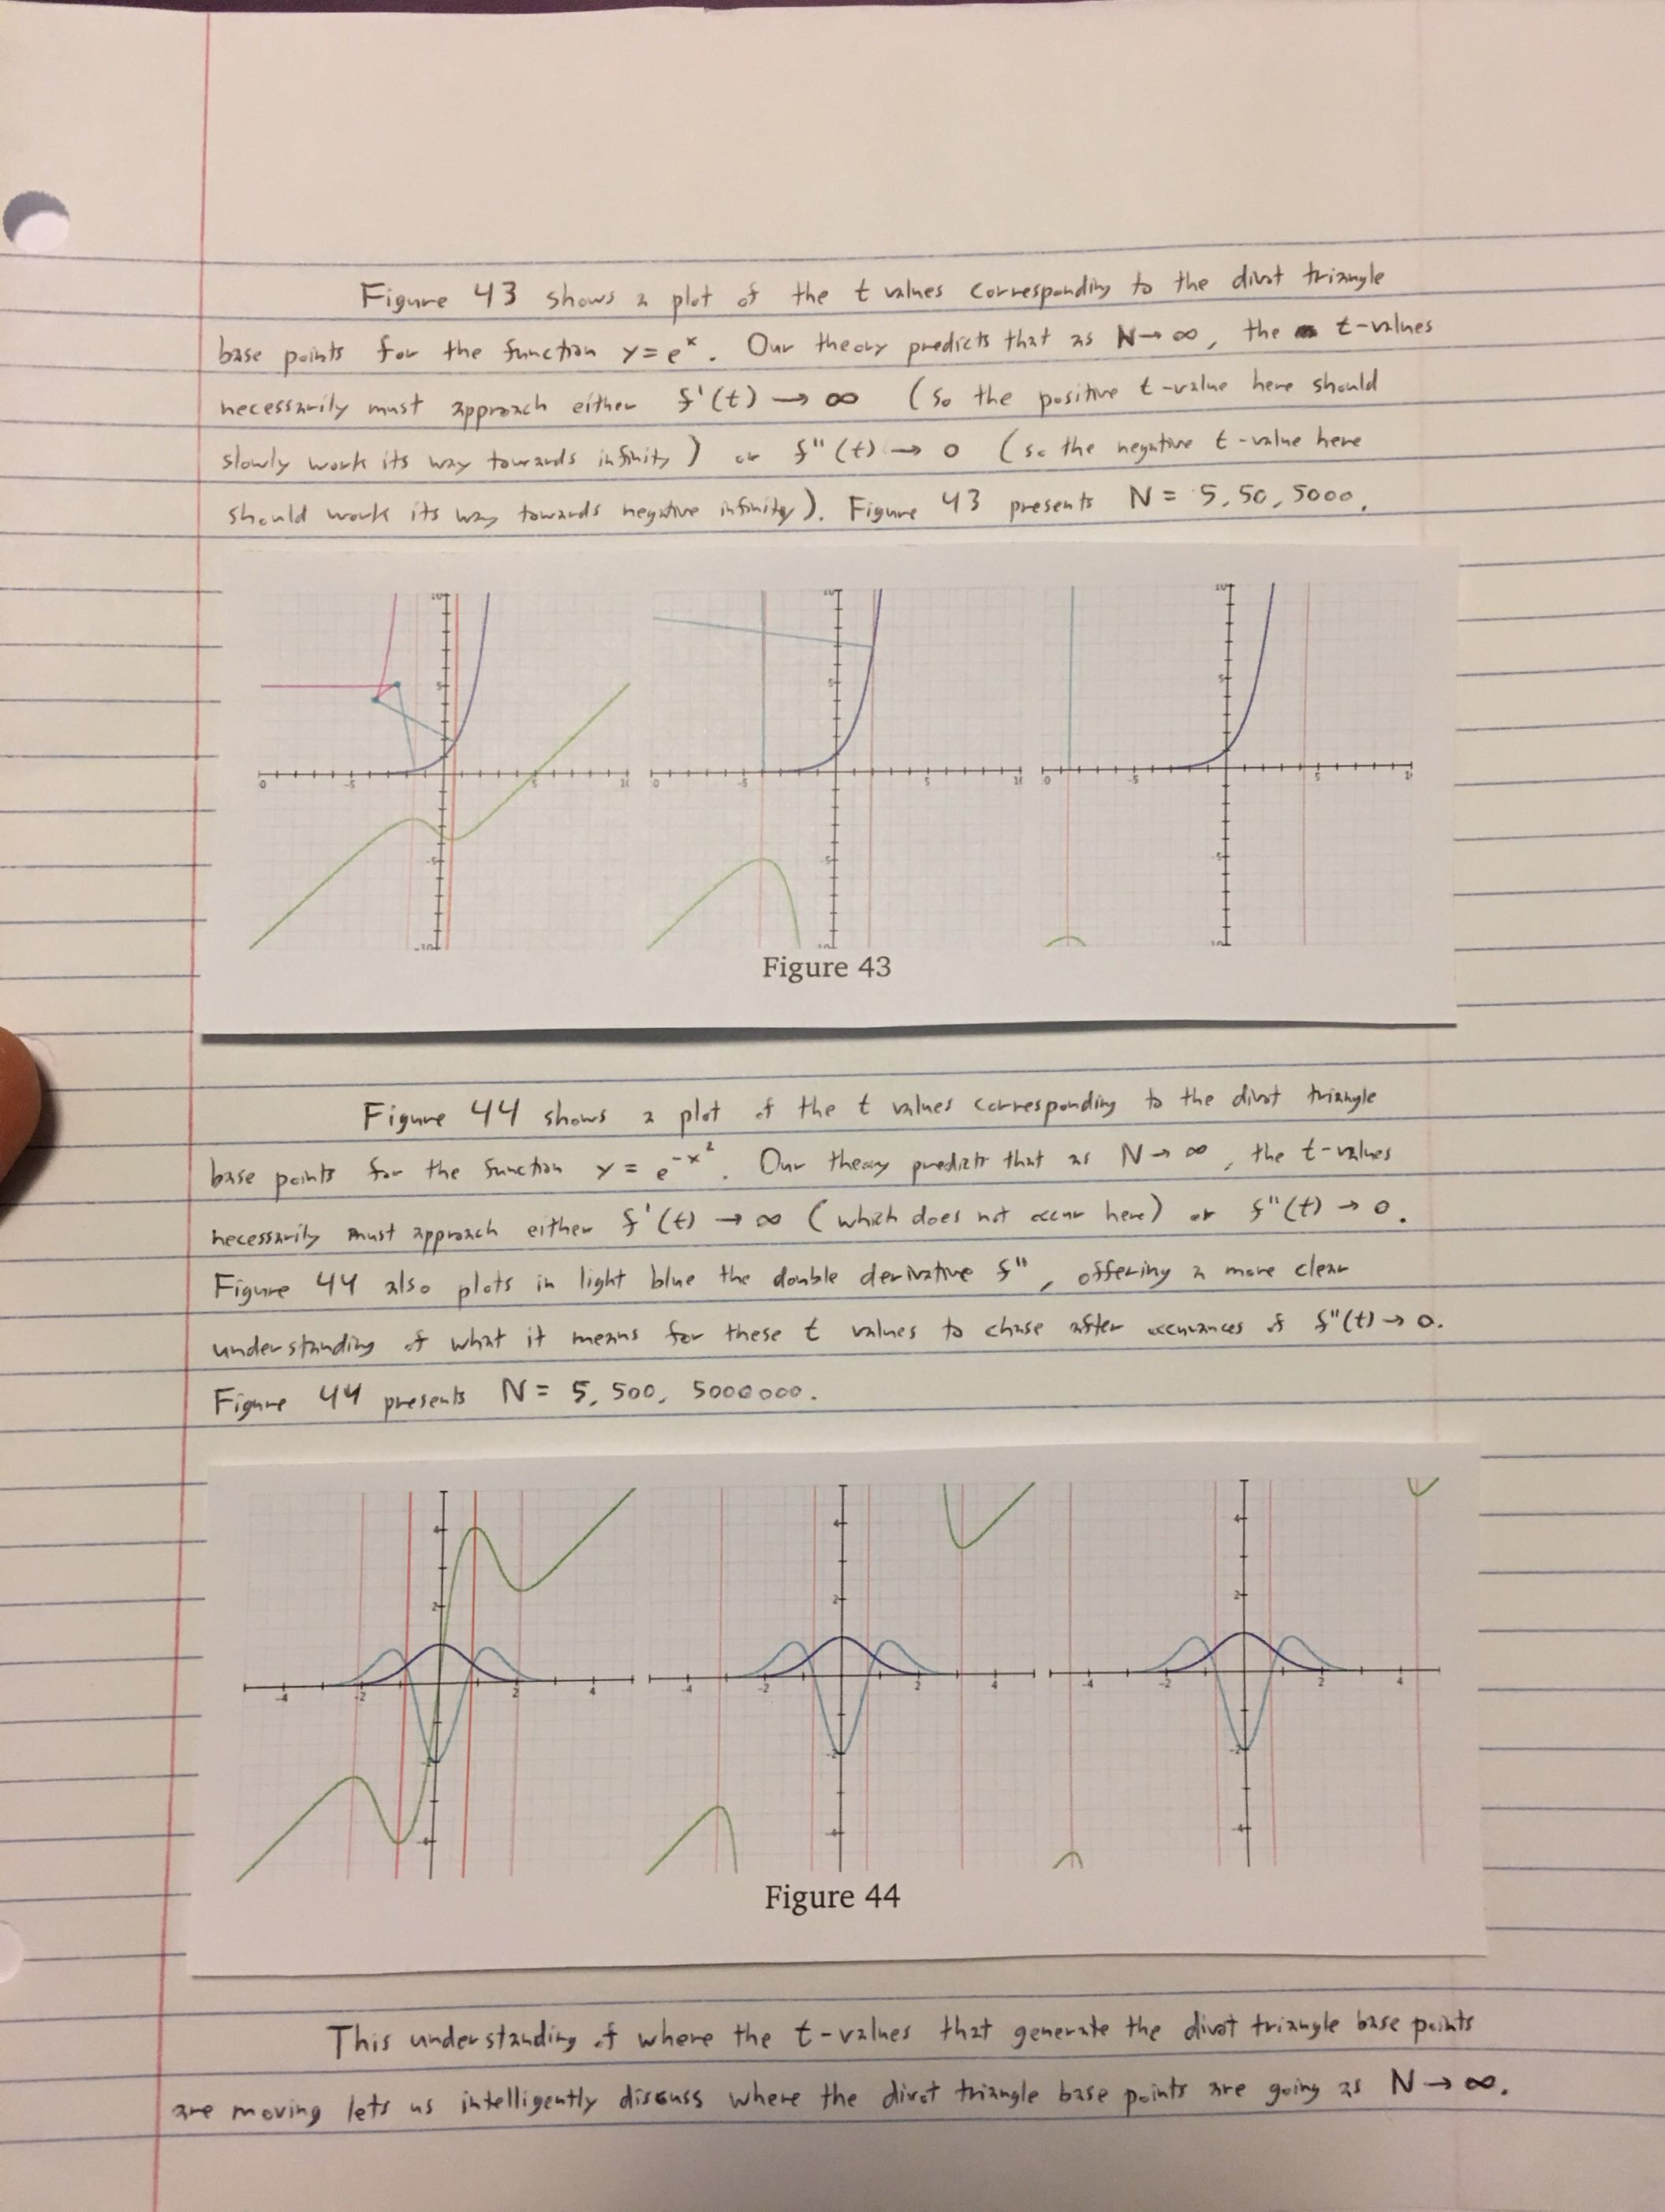
\includegraphics[width=.9\linewidth, height=.25\textheight, keepaspectratio]{solving-divot-paths-img/Fig 12-43.png}
        \caption{Caption}
        \label{fig:fig12-43}
    \end{minipage}
\end{figure}

Figure $\ref{fig:fig12-44}$ shows a plot of the $t$ values corresponding to the divot triangle base points for the function $y = e^{-x^2}$ Our theory predicts that as $N \xrightarrow{} \infty$, the $t$-values necessarily must approach either $f'(t) \xrightarrow{} \infty$ (which does not occur here), or $f''(t) \xrightarrow{} 0$. Figure $\ref{fig:fig12-44}$ also plots in light blue the double derivative $f''$, offering a more clear understanding of what it means for these $t$ values to chase after occurrences of $f''(t) \xrightarrow{} 0$. Figure $\ref{fig:fig12-44}$ presents $N = 5, 500, 5000000$.

\begin{figure}[H]
    \centering
    \begin{minipage}[b]{0.9\linewidth}
        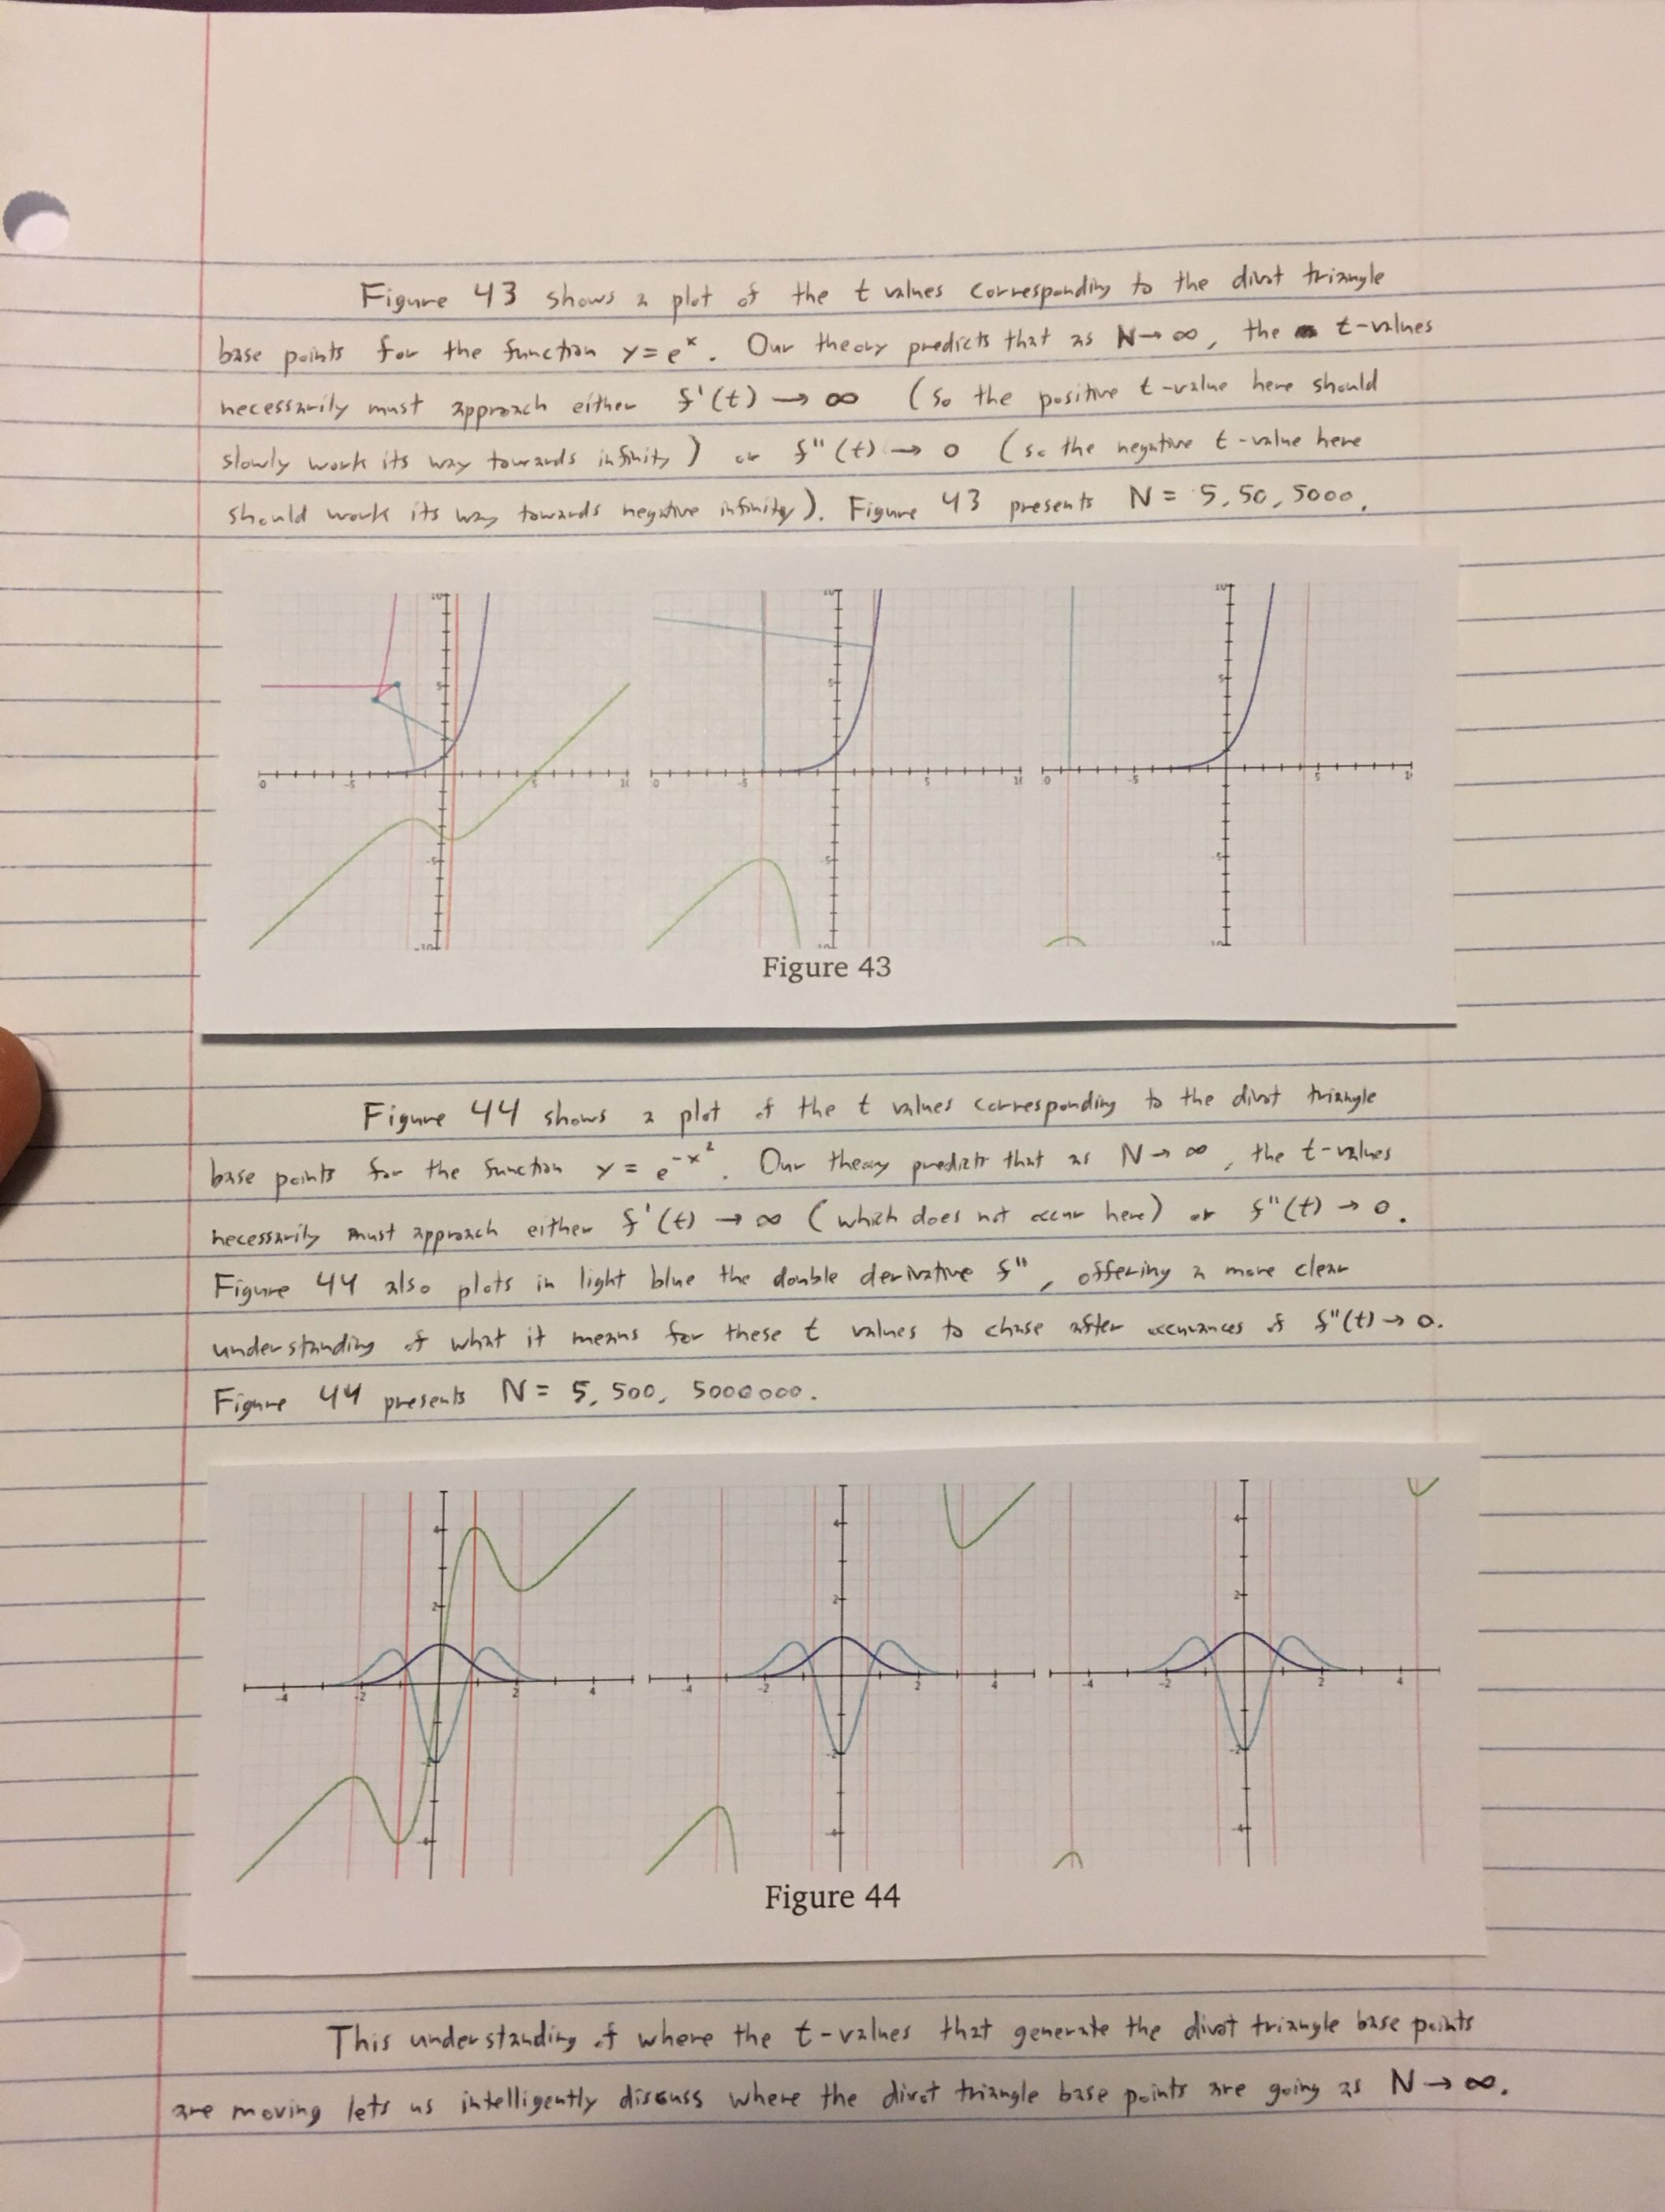
\includegraphics[width=.9\linewidth, height=.25\textheight, keepaspectratio]{solving-divot-paths-img/Fig 12-44.png}
        \caption{Caption}
        \label{fig:fig12-44}
    \end{minipage}
\end{figure}

This understanding of where $t$-values that generate the divot triangle base points are moving lets us intelligently discuss where the triangle base points are going as $N \xrightarrow{} \infty$.

Now we move on in our discussion to the science of divot triangle apex points. Take some function $y = f(x)$ twice differentiable whose second derivative is continuous.  When $N$ is 0, $f_N(t)$ will have no crunch point. If you begin raising or lowering the value of $N$, however, so long as $f(x)$ has any twists or turns at all and is not a perfectly straight line on all $x \in \mathbb{R}$. we will find crunch spots. These will occur at very particular values of $N$, spawning the birth of divot triangles.

\begin{wrapfigure}{l}{0.25\textwidth}
  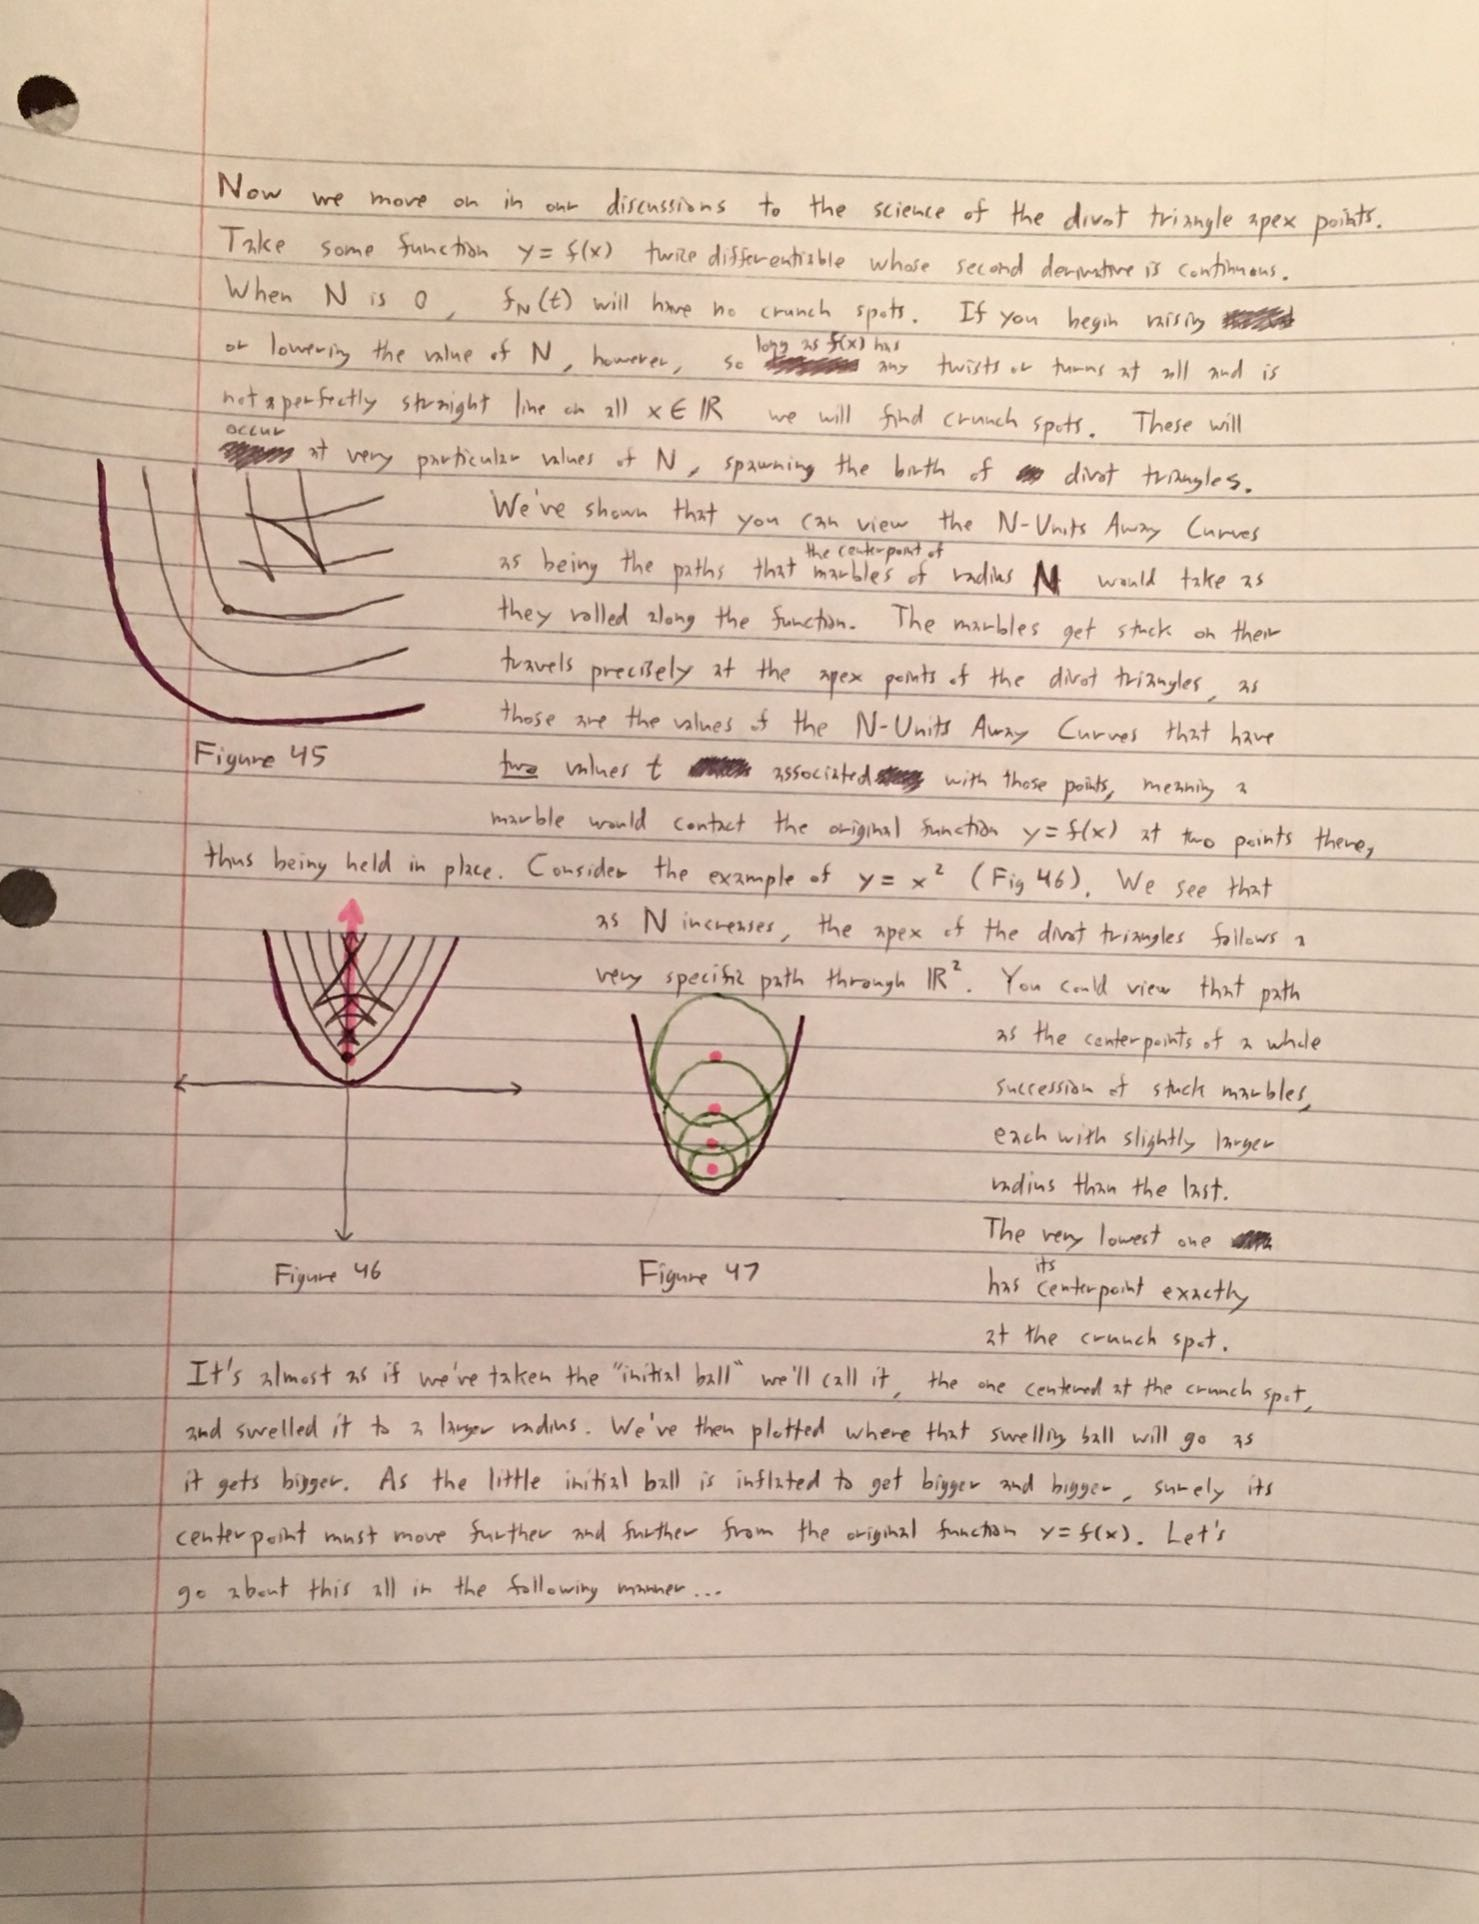
\includegraphics[width=.9\linewidth]{solving-divot-paths-img/Fig 12-45.png}
  \caption{Caption}
  \label{fig:fig12-45}
\end{wrapfigure}

We've shown that you can view the $N$-Units Away Curves as being the paths that the centerpoint of marbles of radius $N$ would take as they rolled along the function. The marbles get stuck on their travels precisely at the apex points of the divot triangles, as those are the values of the $N$-Units Away Curves that have \textit{two} values $t$ associated with those points, meaning a marble would contact the original function $y = f(x)$ at two points there, thus being held in place. Consider the example of $y = x^2$ (Fig $\ref{fig:fig12-46}$. We see that as $N$ increases, the apex of the divot triangles follow a very specific path through $\mathbb{R}^2$. You could view that path as the centerpoints of a while succession of stuck marbles, each with slightly larger radius than the last. The very lowest one has its centerpoint exactly at the crunch spot.

It's almost as if we've taken the ``initial ball'' we'll call it, the one centered at the crunch spot, ans swelled it to a larger radius. We've then plotted where that swelling ball will go as it gets bigger. As the little initial ball is inflated to get bigger and bigger, surely its centerpoint must move further and further from the original function $y = f(x)$. Let's go about this n the following manner...

\begin{figure}[H]
    \centering
    \begin{minipage}[b]{0.5\linewidth}
        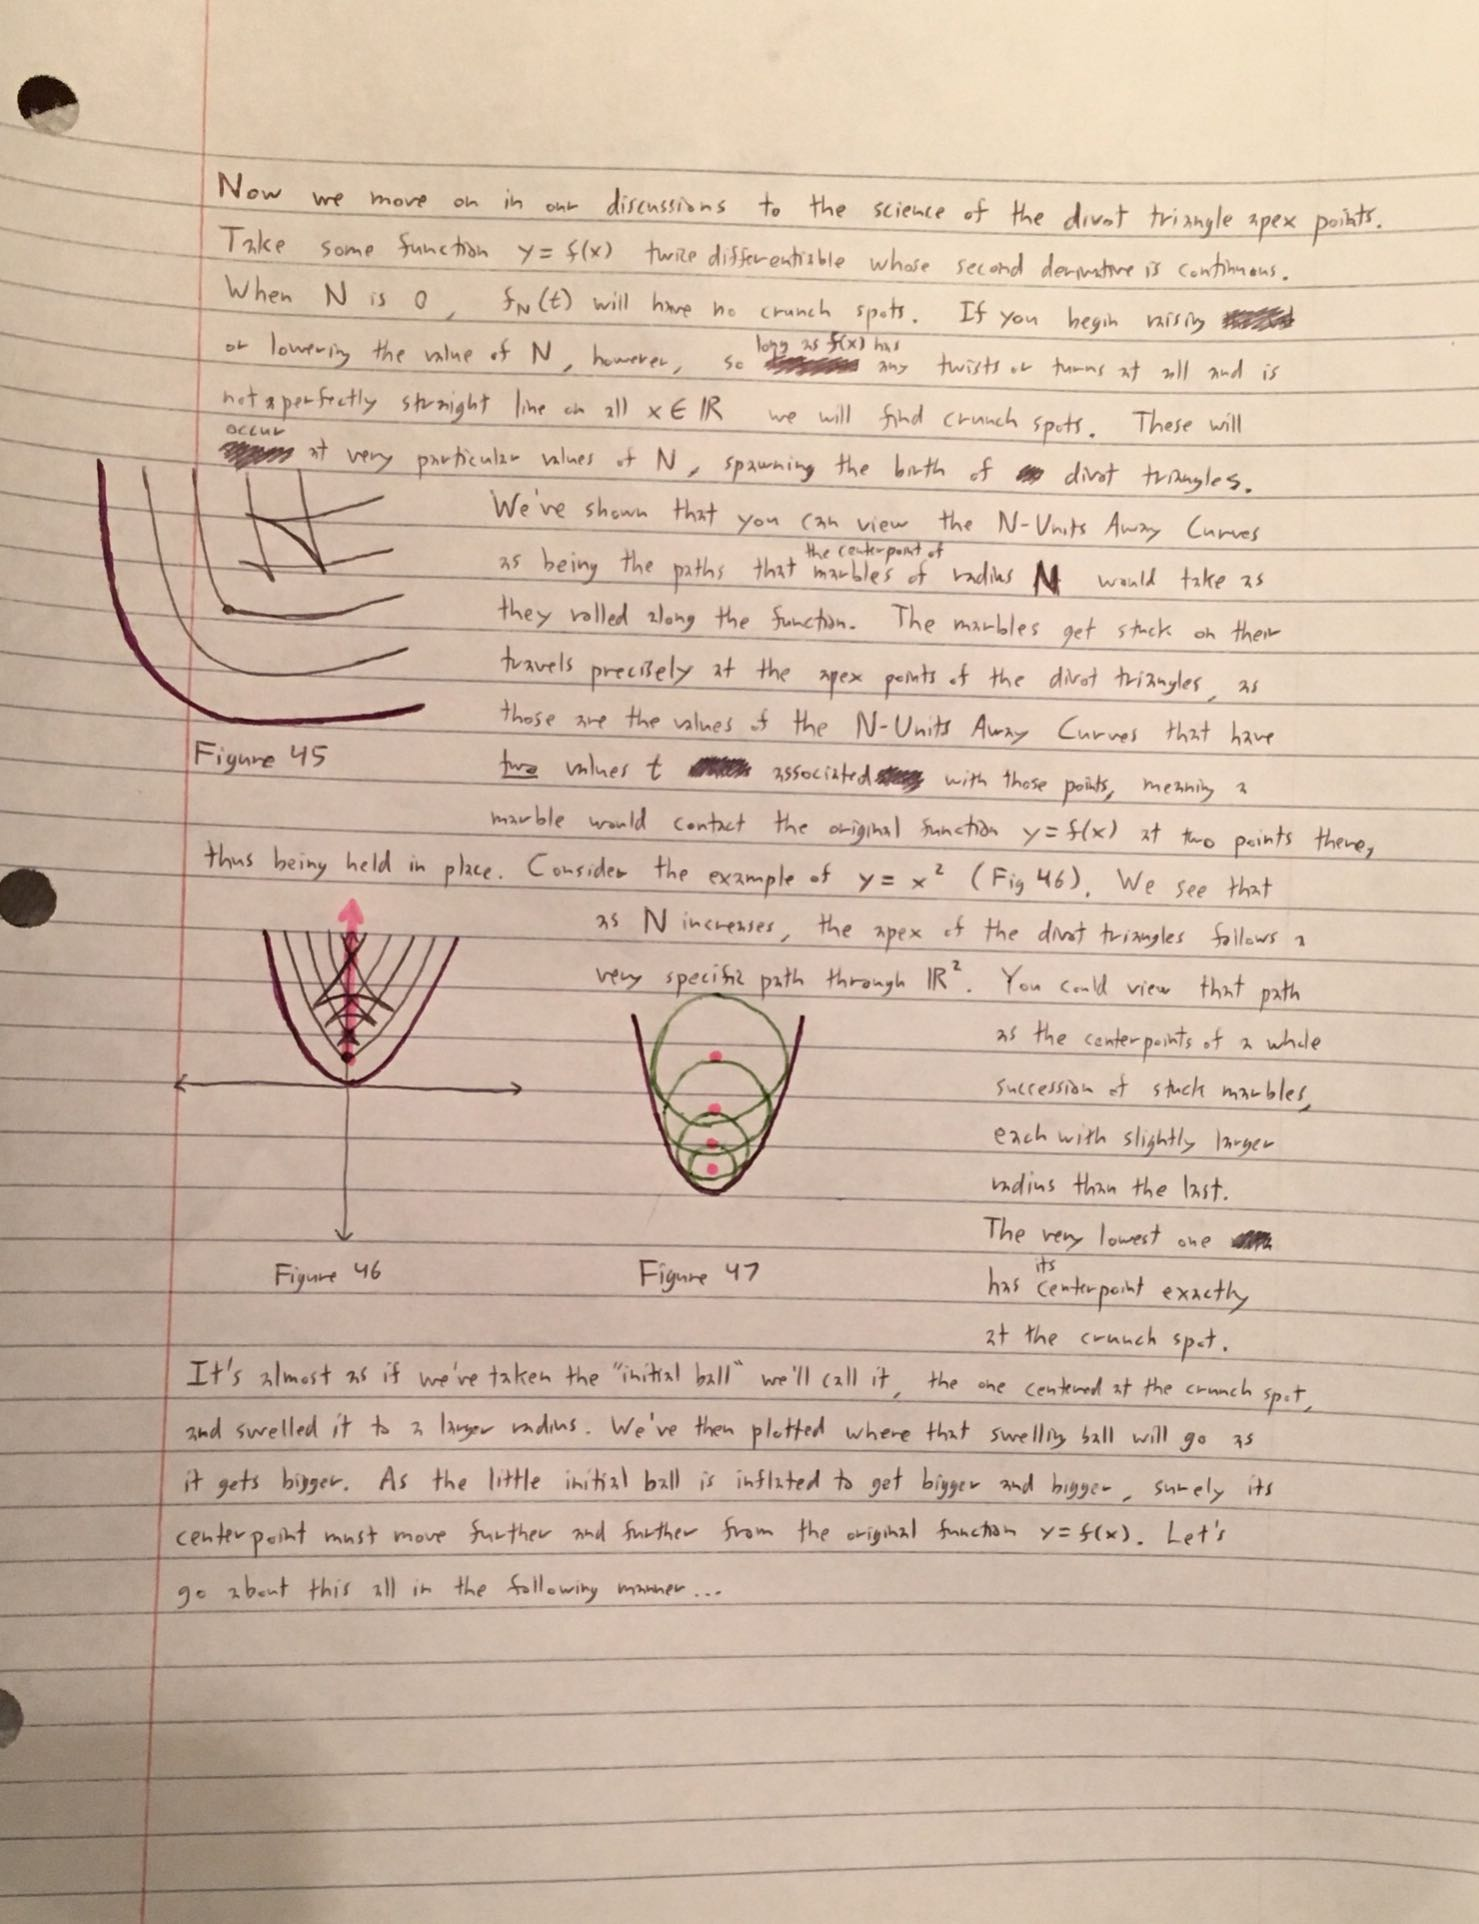
\includegraphics[width=.9\linewidth]{solving-divot-paths-img/Fig 12-46.png}
        \caption{Caption}
        \label{fig:fig12-46}
    \end{minipage}
    \begin{minipage}[b]{0.5\linewidth}
        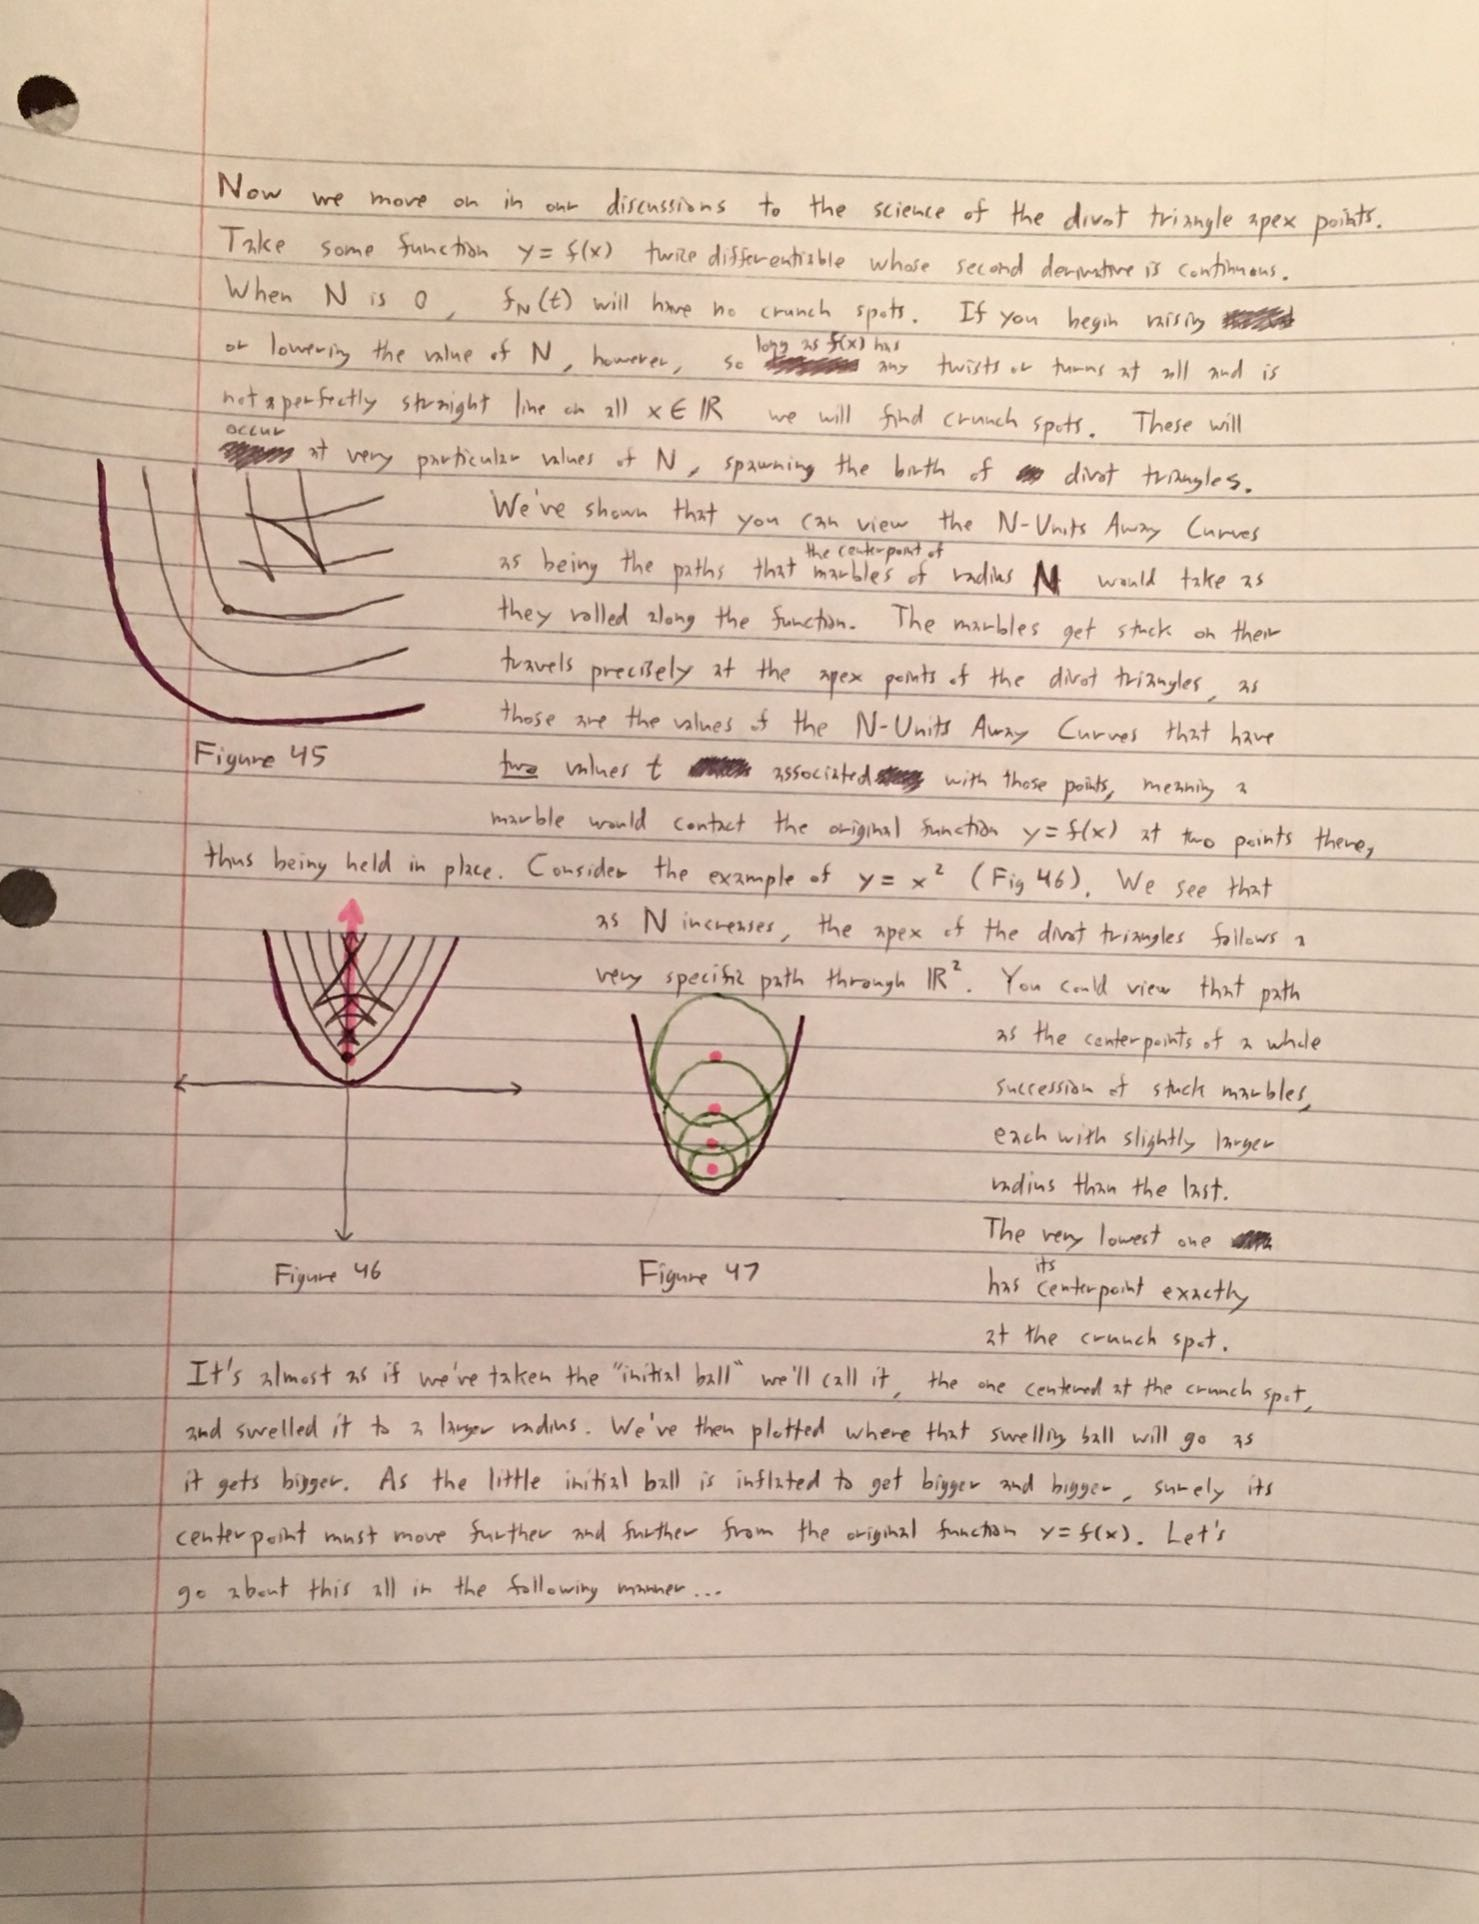
\includegraphics[width=.9\linewidth]{solving-divot-paths-img/Fig 12-47.png}
        \caption{Caption}
        \label{fig:fig12-47}
    \end{minipage}
\end{figure}

Choose a function $y = f(x)$. Find a crunch spot for that function.

\begin{wrapfigure}{l}{0.25\textwidth}
  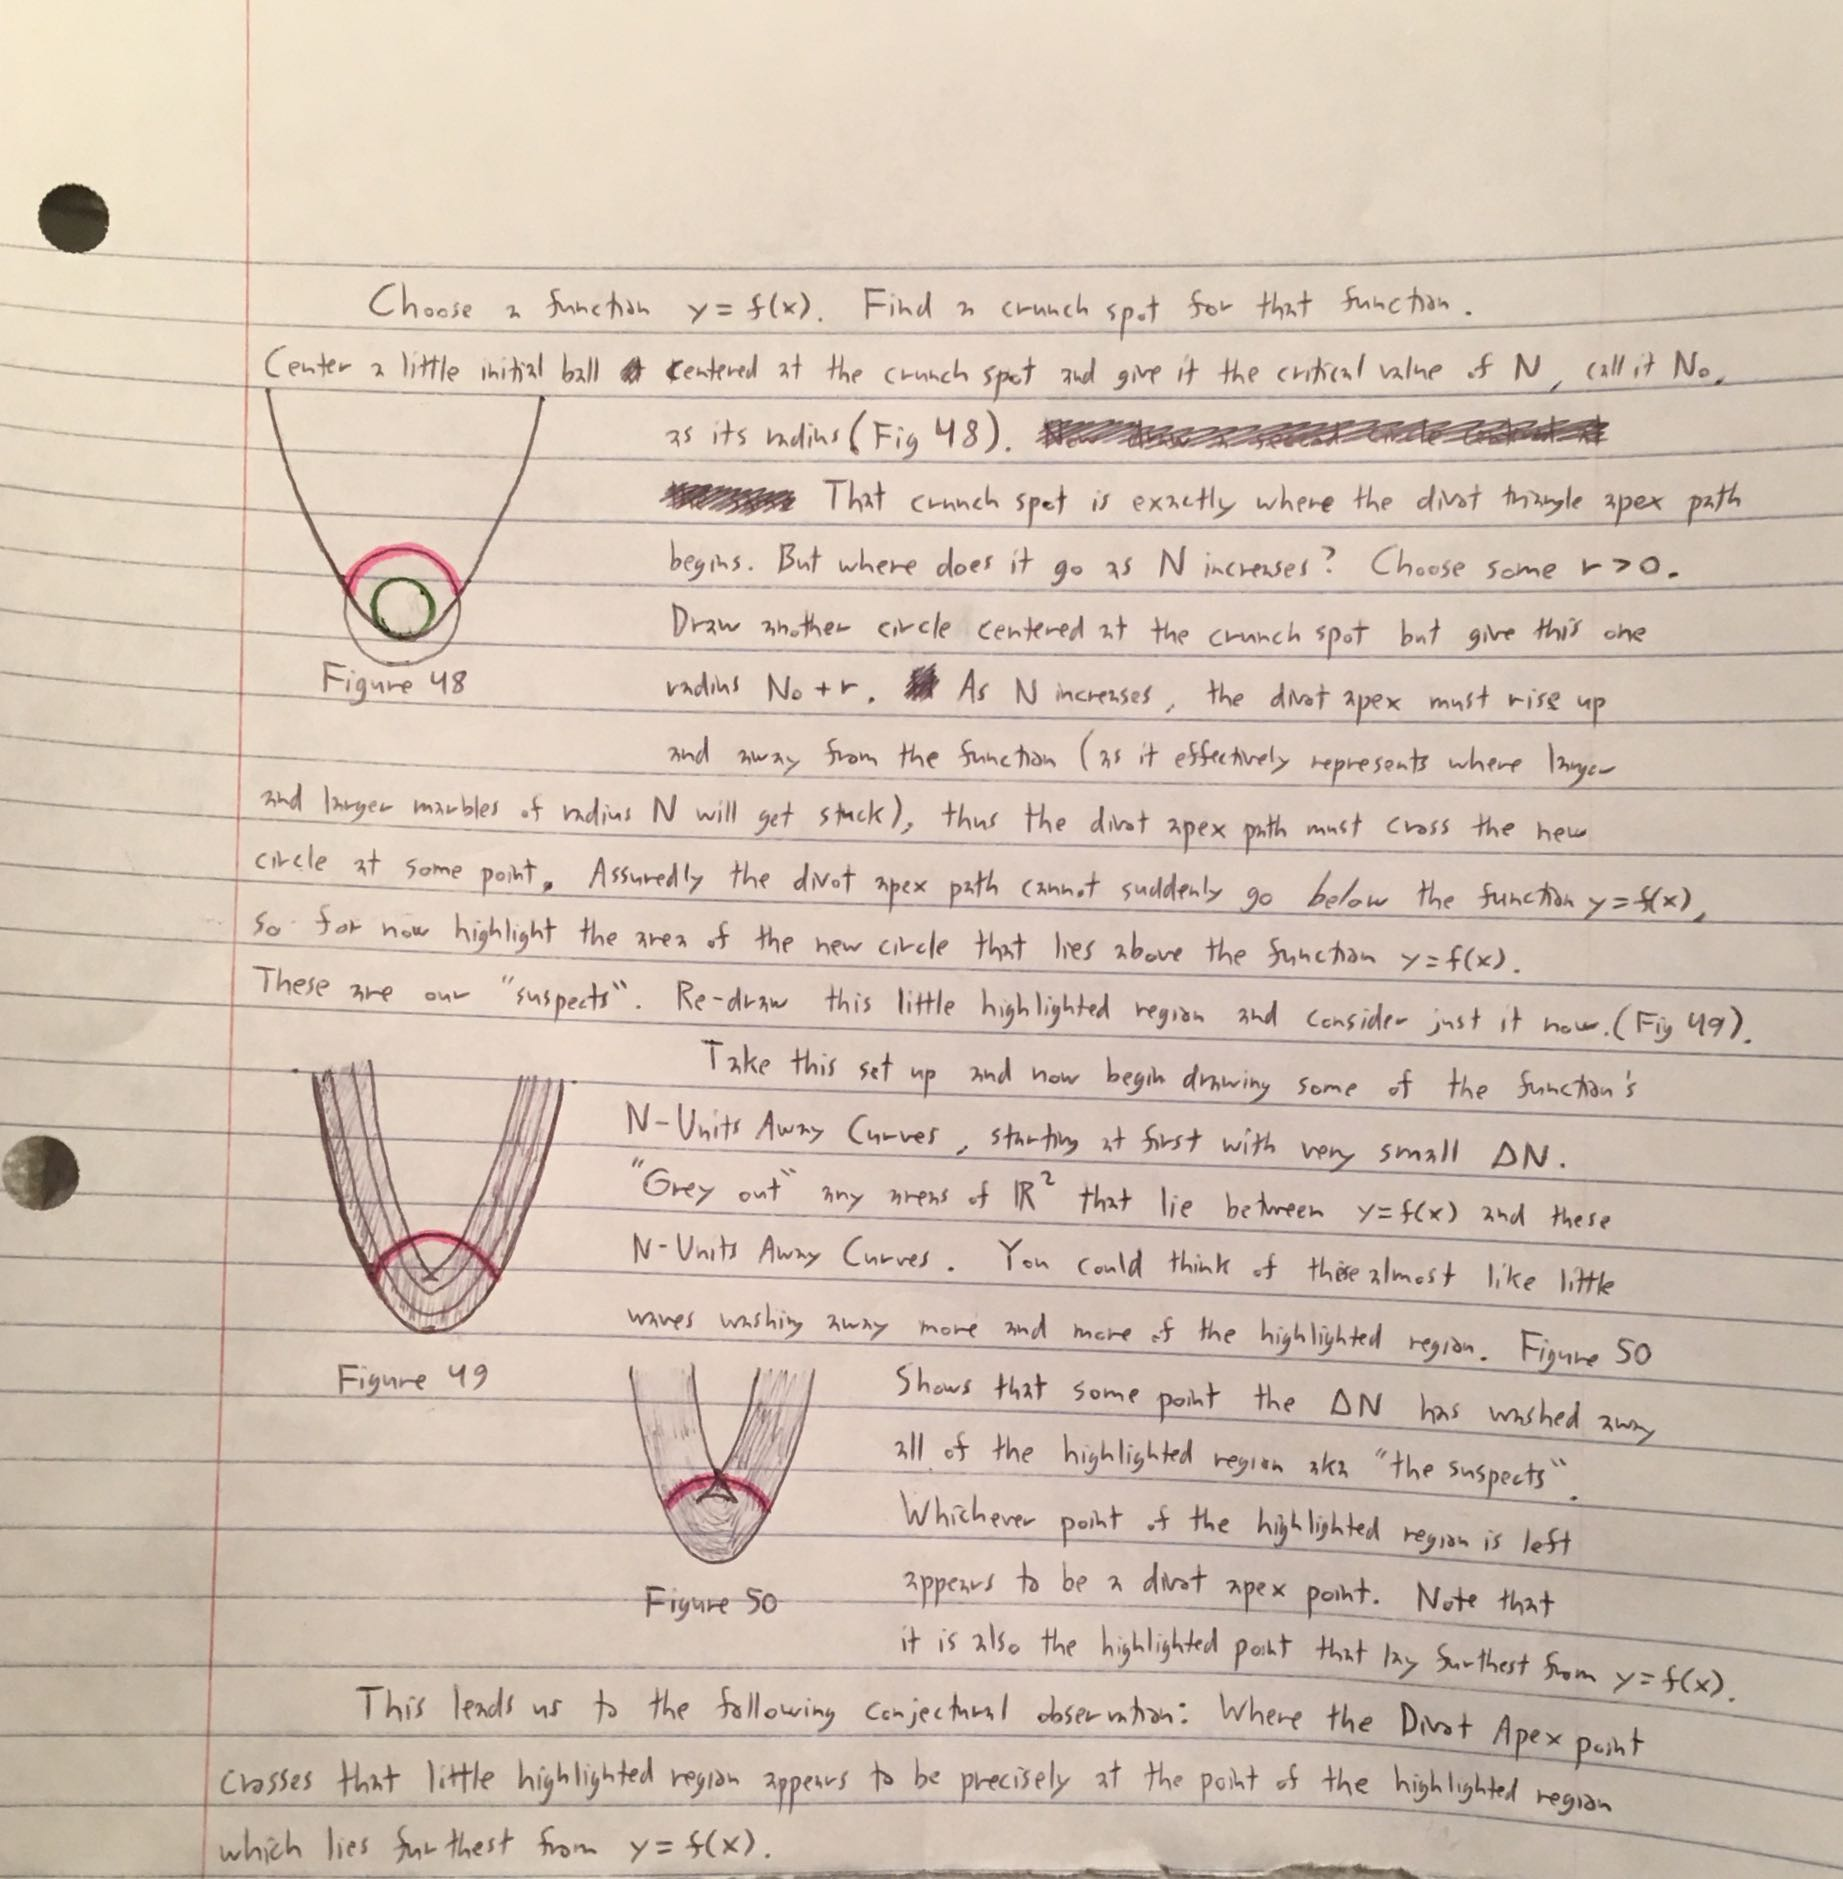
\includegraphics[width=.9\linewidth]{solving-divot-paths-img/Fig 12-48.png}
  \caption{Caption}
  \label{fig:fig12-48}
\end{wrapfigure}

Center a little initial ball at the crunch spot and give it the critical value of $N$, call it $N_o$, as its radius (Fig $\ref{fig:fig12-48}$. That crunch spot is exactly where the divot triangle apex path begins. But where does it go as $N$ increases? Choose some $r > 0$. Draw another circles centered at the crunch spot but give this one radius $N_o + r$. As $N$ increases, the divot apex must rise up and away from the function (as it effectively represents where larger and larger marbles of radius $N$ will get stuck), thus the divot apex path must cross the new circle at some point. Assuredly the divot apex path cannot suddenly go \textit{below} the function $y = f(x)$, so for now highlight the area of the new circle that lies above the function $y = f(x)$.

\begin{wrapfigure}{l}{0.25\textwidth}
  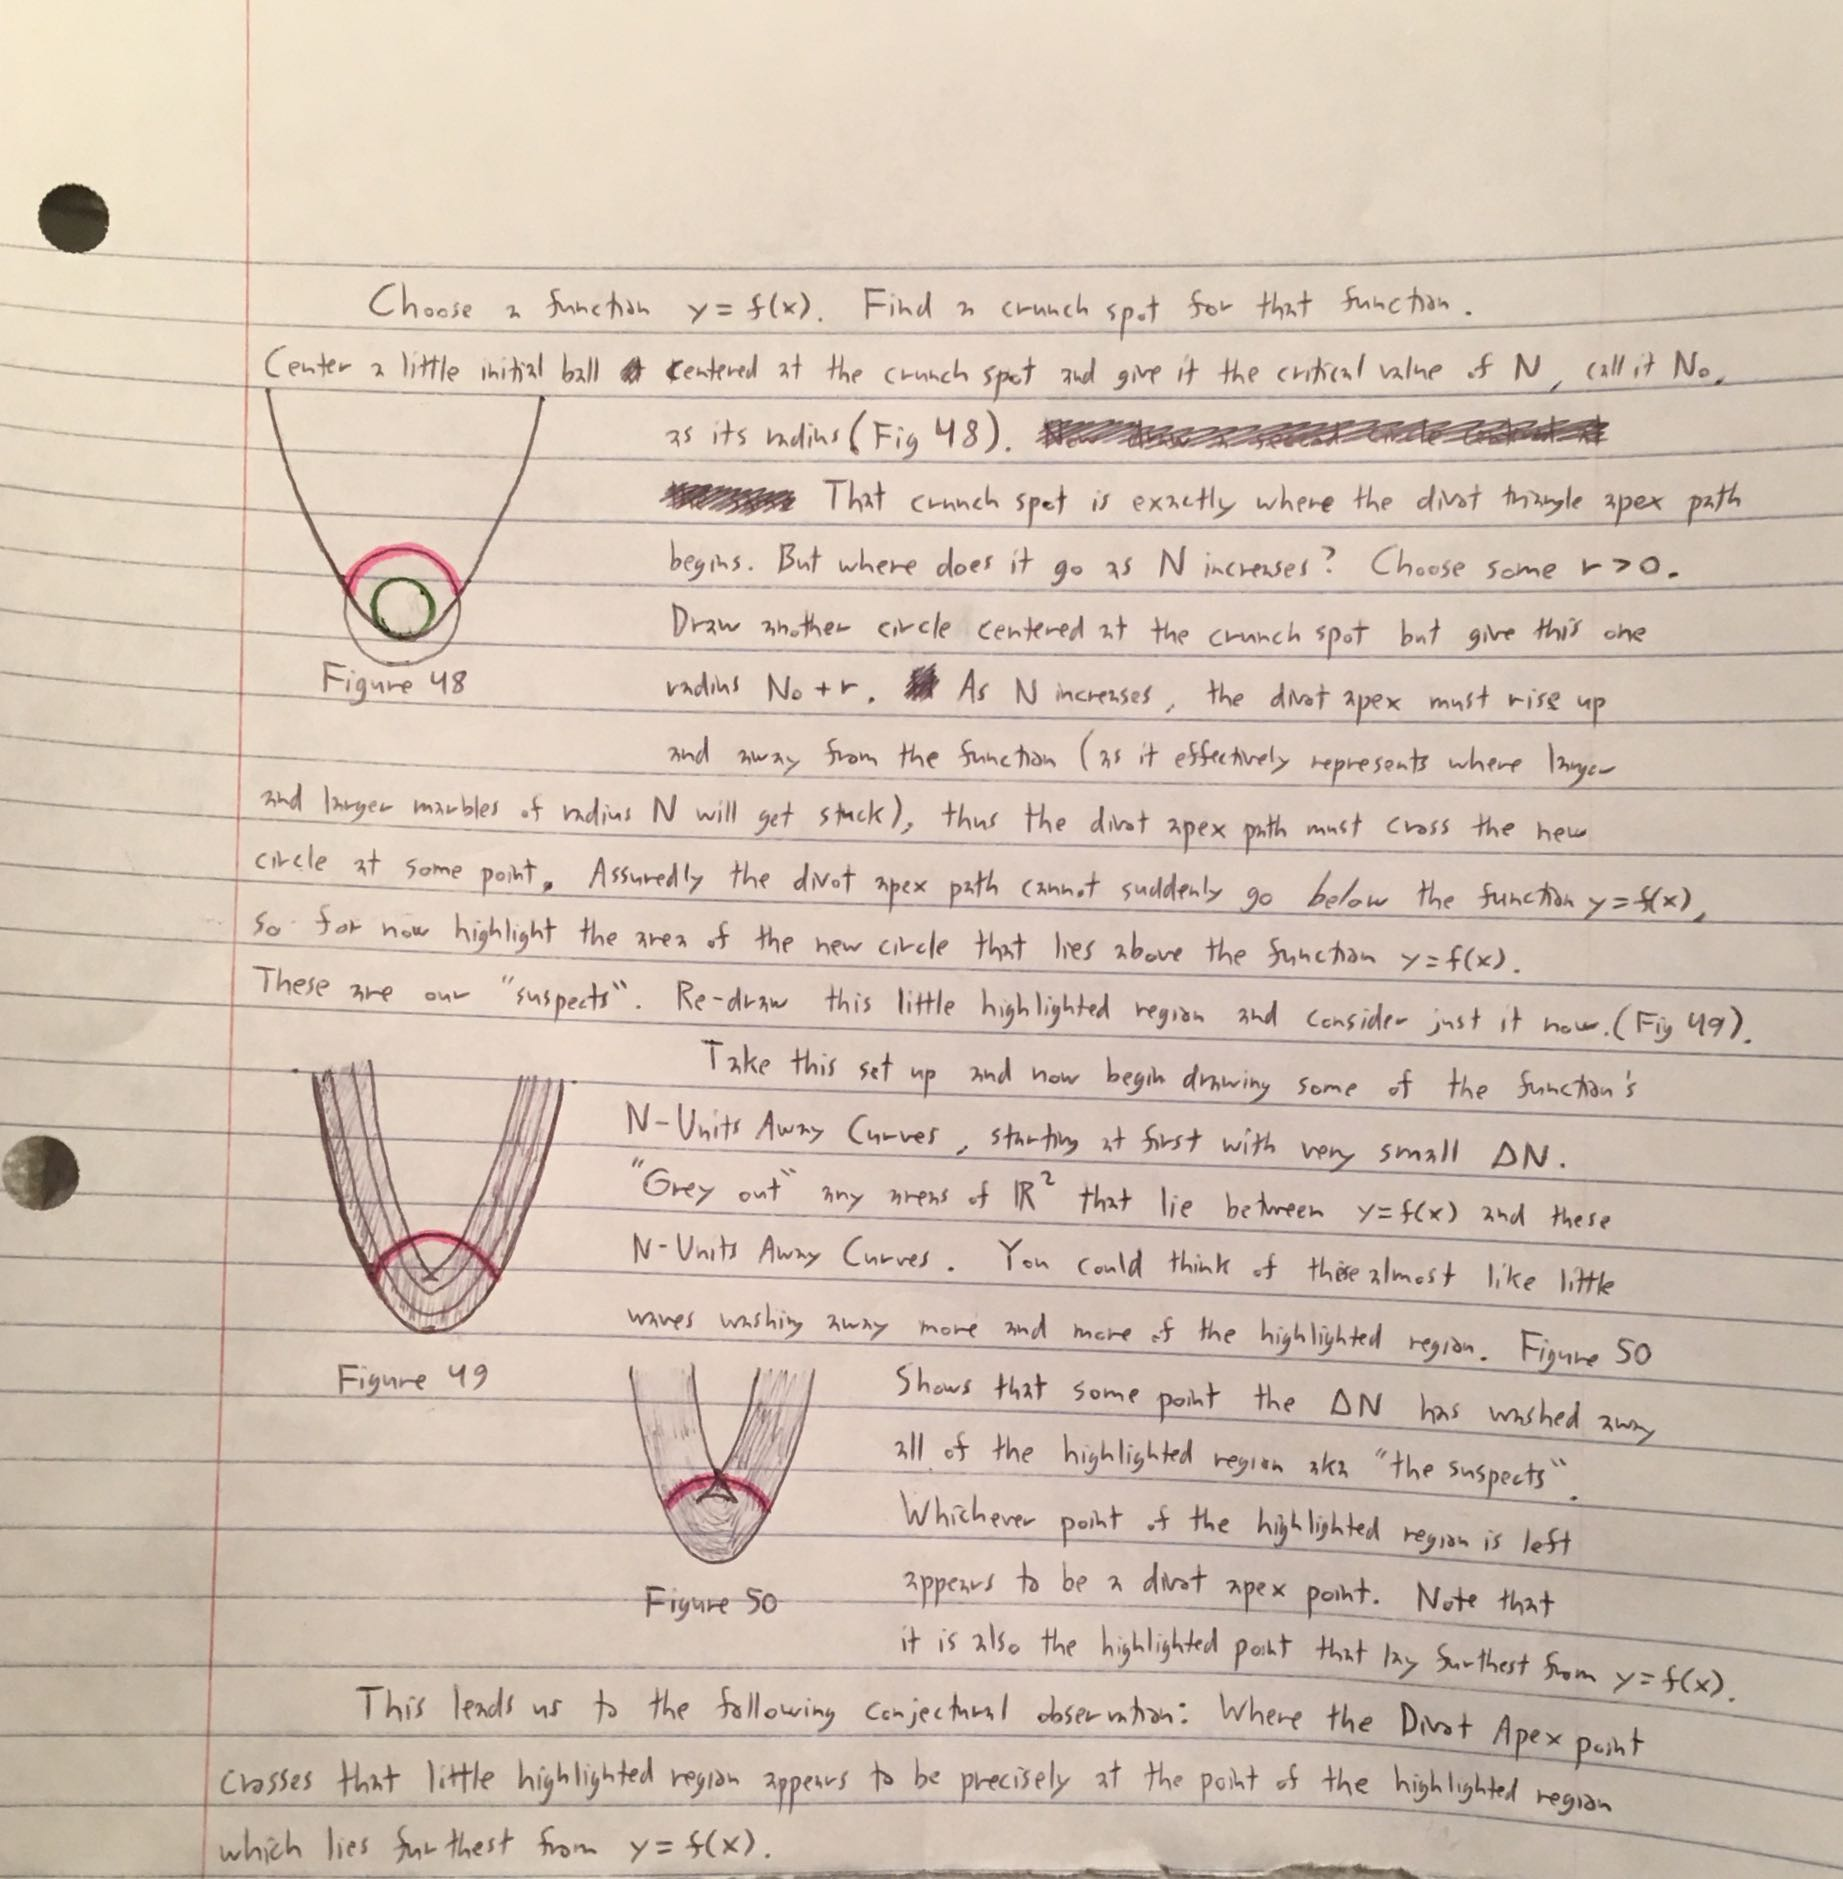
\includegraphics[width=.9\linewidth]{solving-divot-paths-img/Fig 12-49.png}
  \caption{Caption}
  \label{fig:fig12-49}
\end{wrapfigure}

These are our ``suspect''. Re-draw this little highlighted region and consider just it now. (Fig $\ref{fig:fig12-49}$. Take this set up and now begin drawing some of the function's $N$-Units Away Curves, starting at first with very small $ \Delta N$. ``Grey out'' any areas of $\mathbb{R} ^ 2$ that lie between $y = f(x)$ and these $N$-Units Away Curves. You could think of these almost like little waces washing away more and more of the highlighted region. Figure $\ref{fig:fig12-50}$ shows that some point the $\Delta N$ has washed away all of the highlighted region aka ``the suspects''. 

\begin{wrapfigure}{l}{0.25\textwidth}
  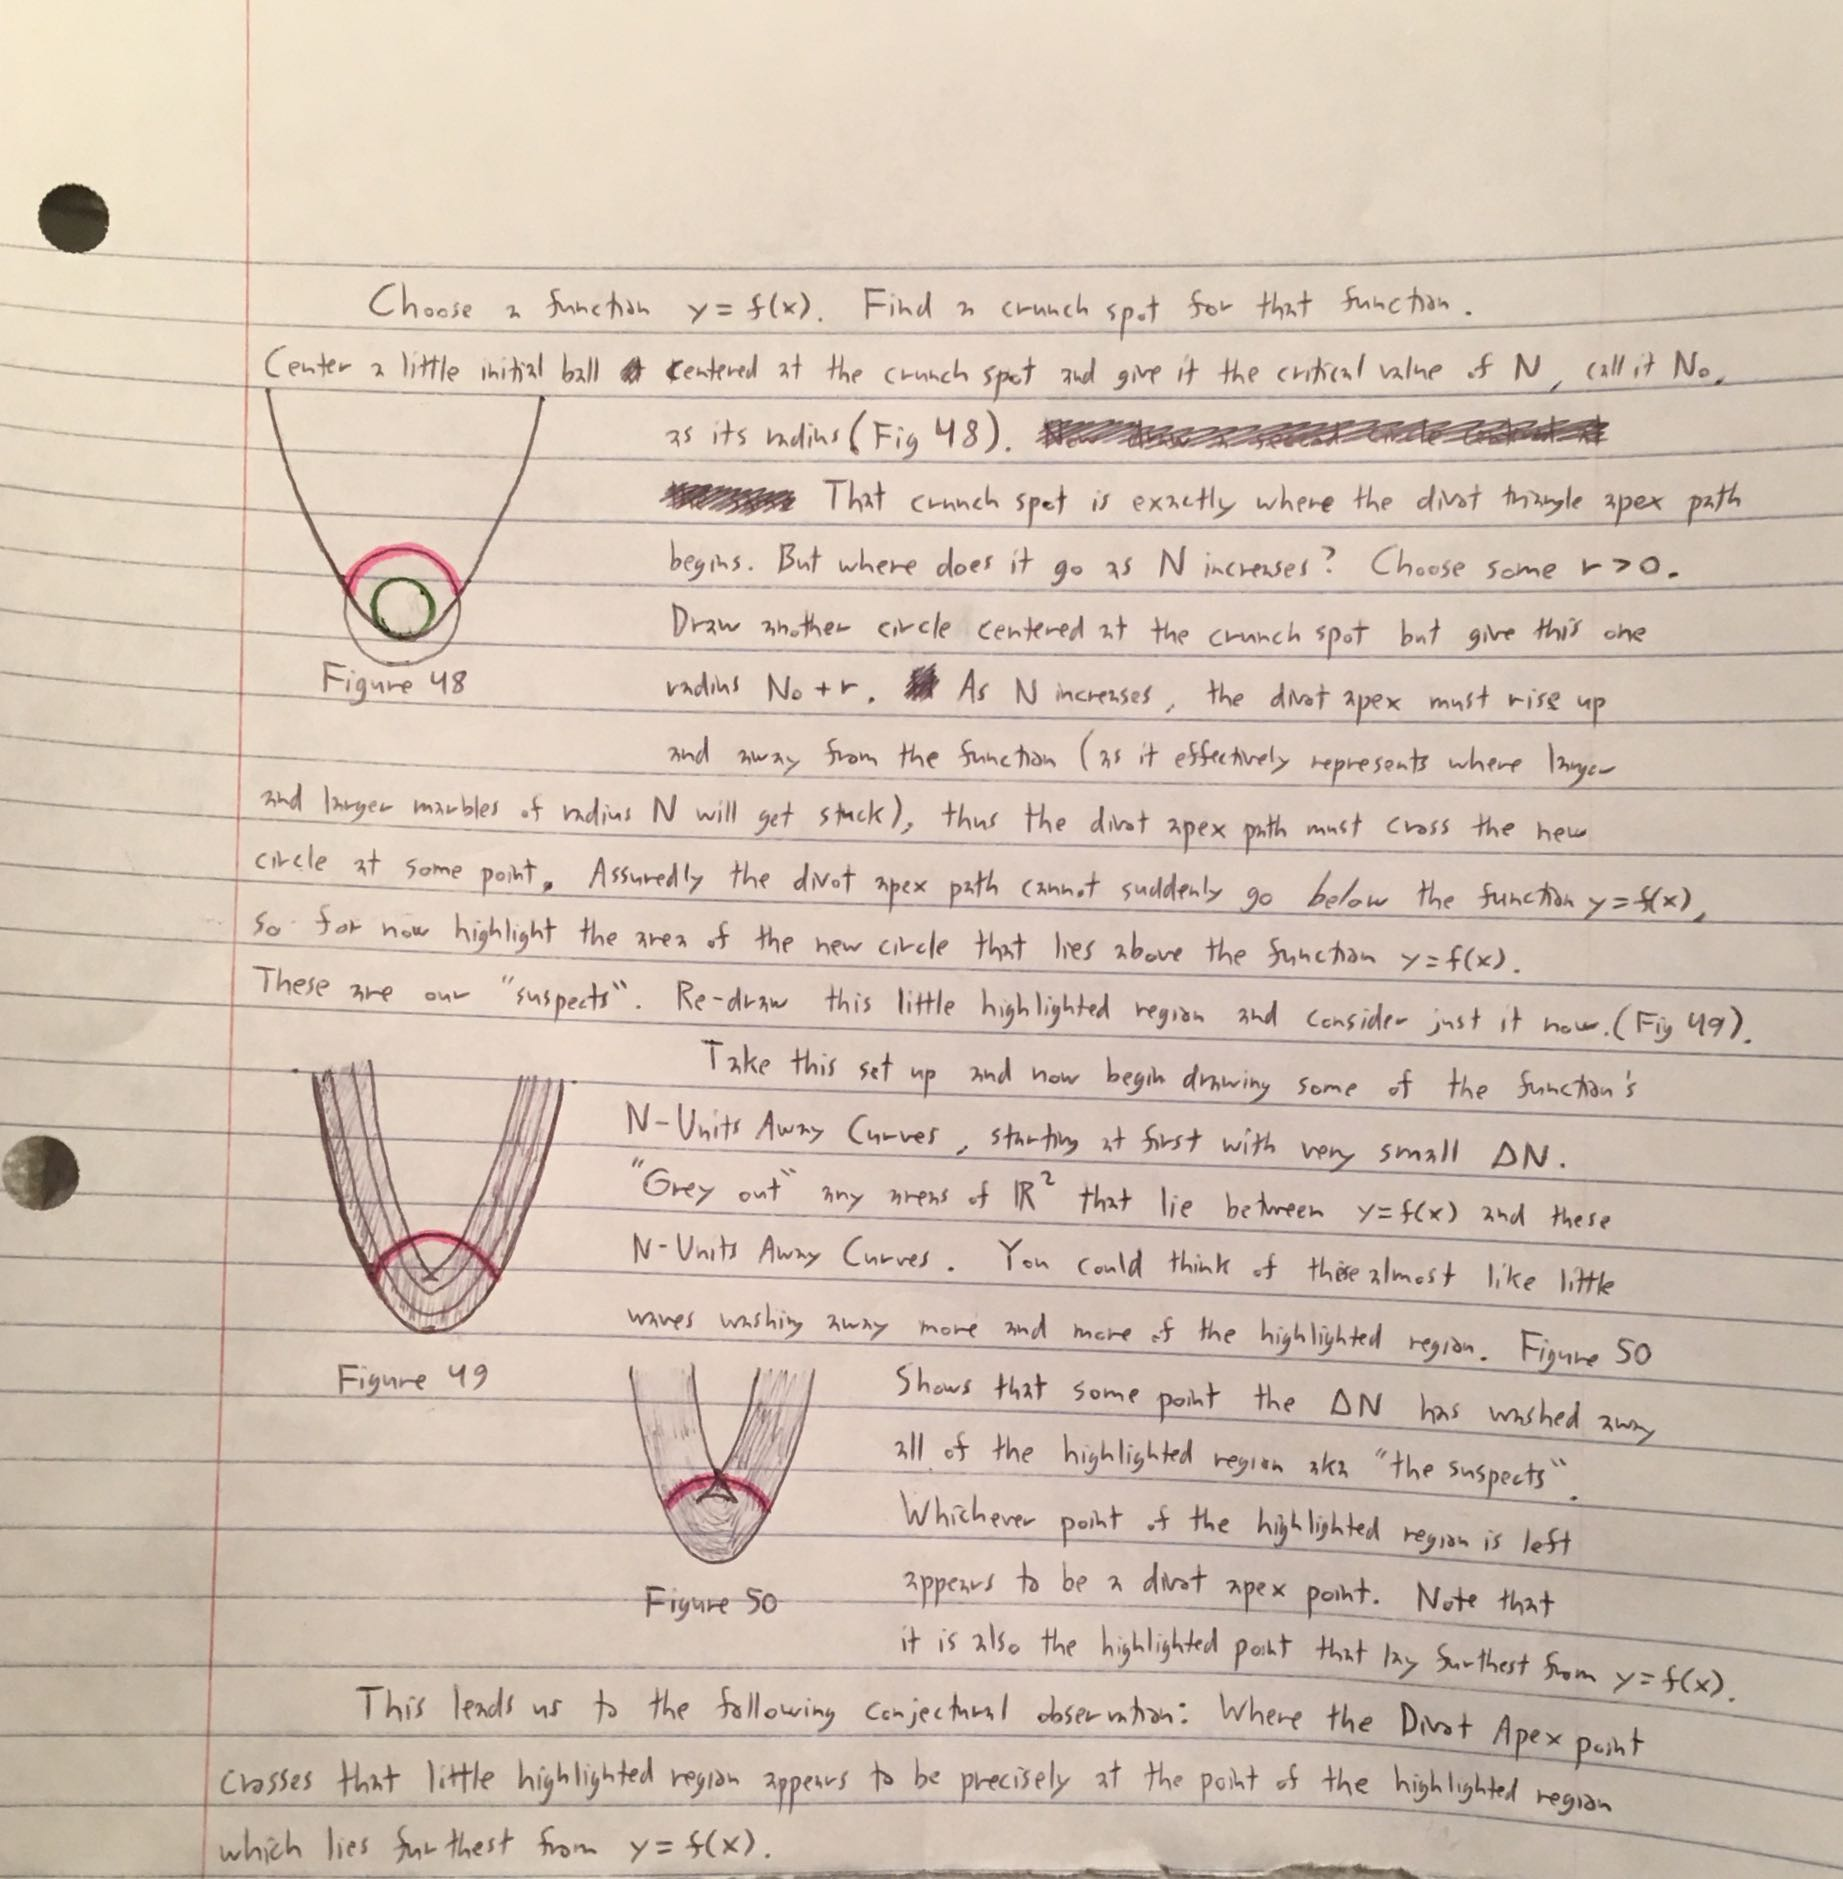
\includegraphics[width=.9\linewidth]{solving-divot-paths-img/Fig 12-50.png}
  \caption{Caption}
  \label{fig:fig12-50}
\end{wrapfigure}

Whichever point of the highlighted region is left appears to be a divot apex point. Note that it is also the highlighted point that lay furthest from $y = f(x)$. This leads us to the following conjectural observation: Where the Divot Apex point crosses that little highlighted region appears to be precisely at the point of the highlighted region which lies furthest from $y = f(x)$.

\begin{wrapfigure}{l}{0.25\textwidth}
  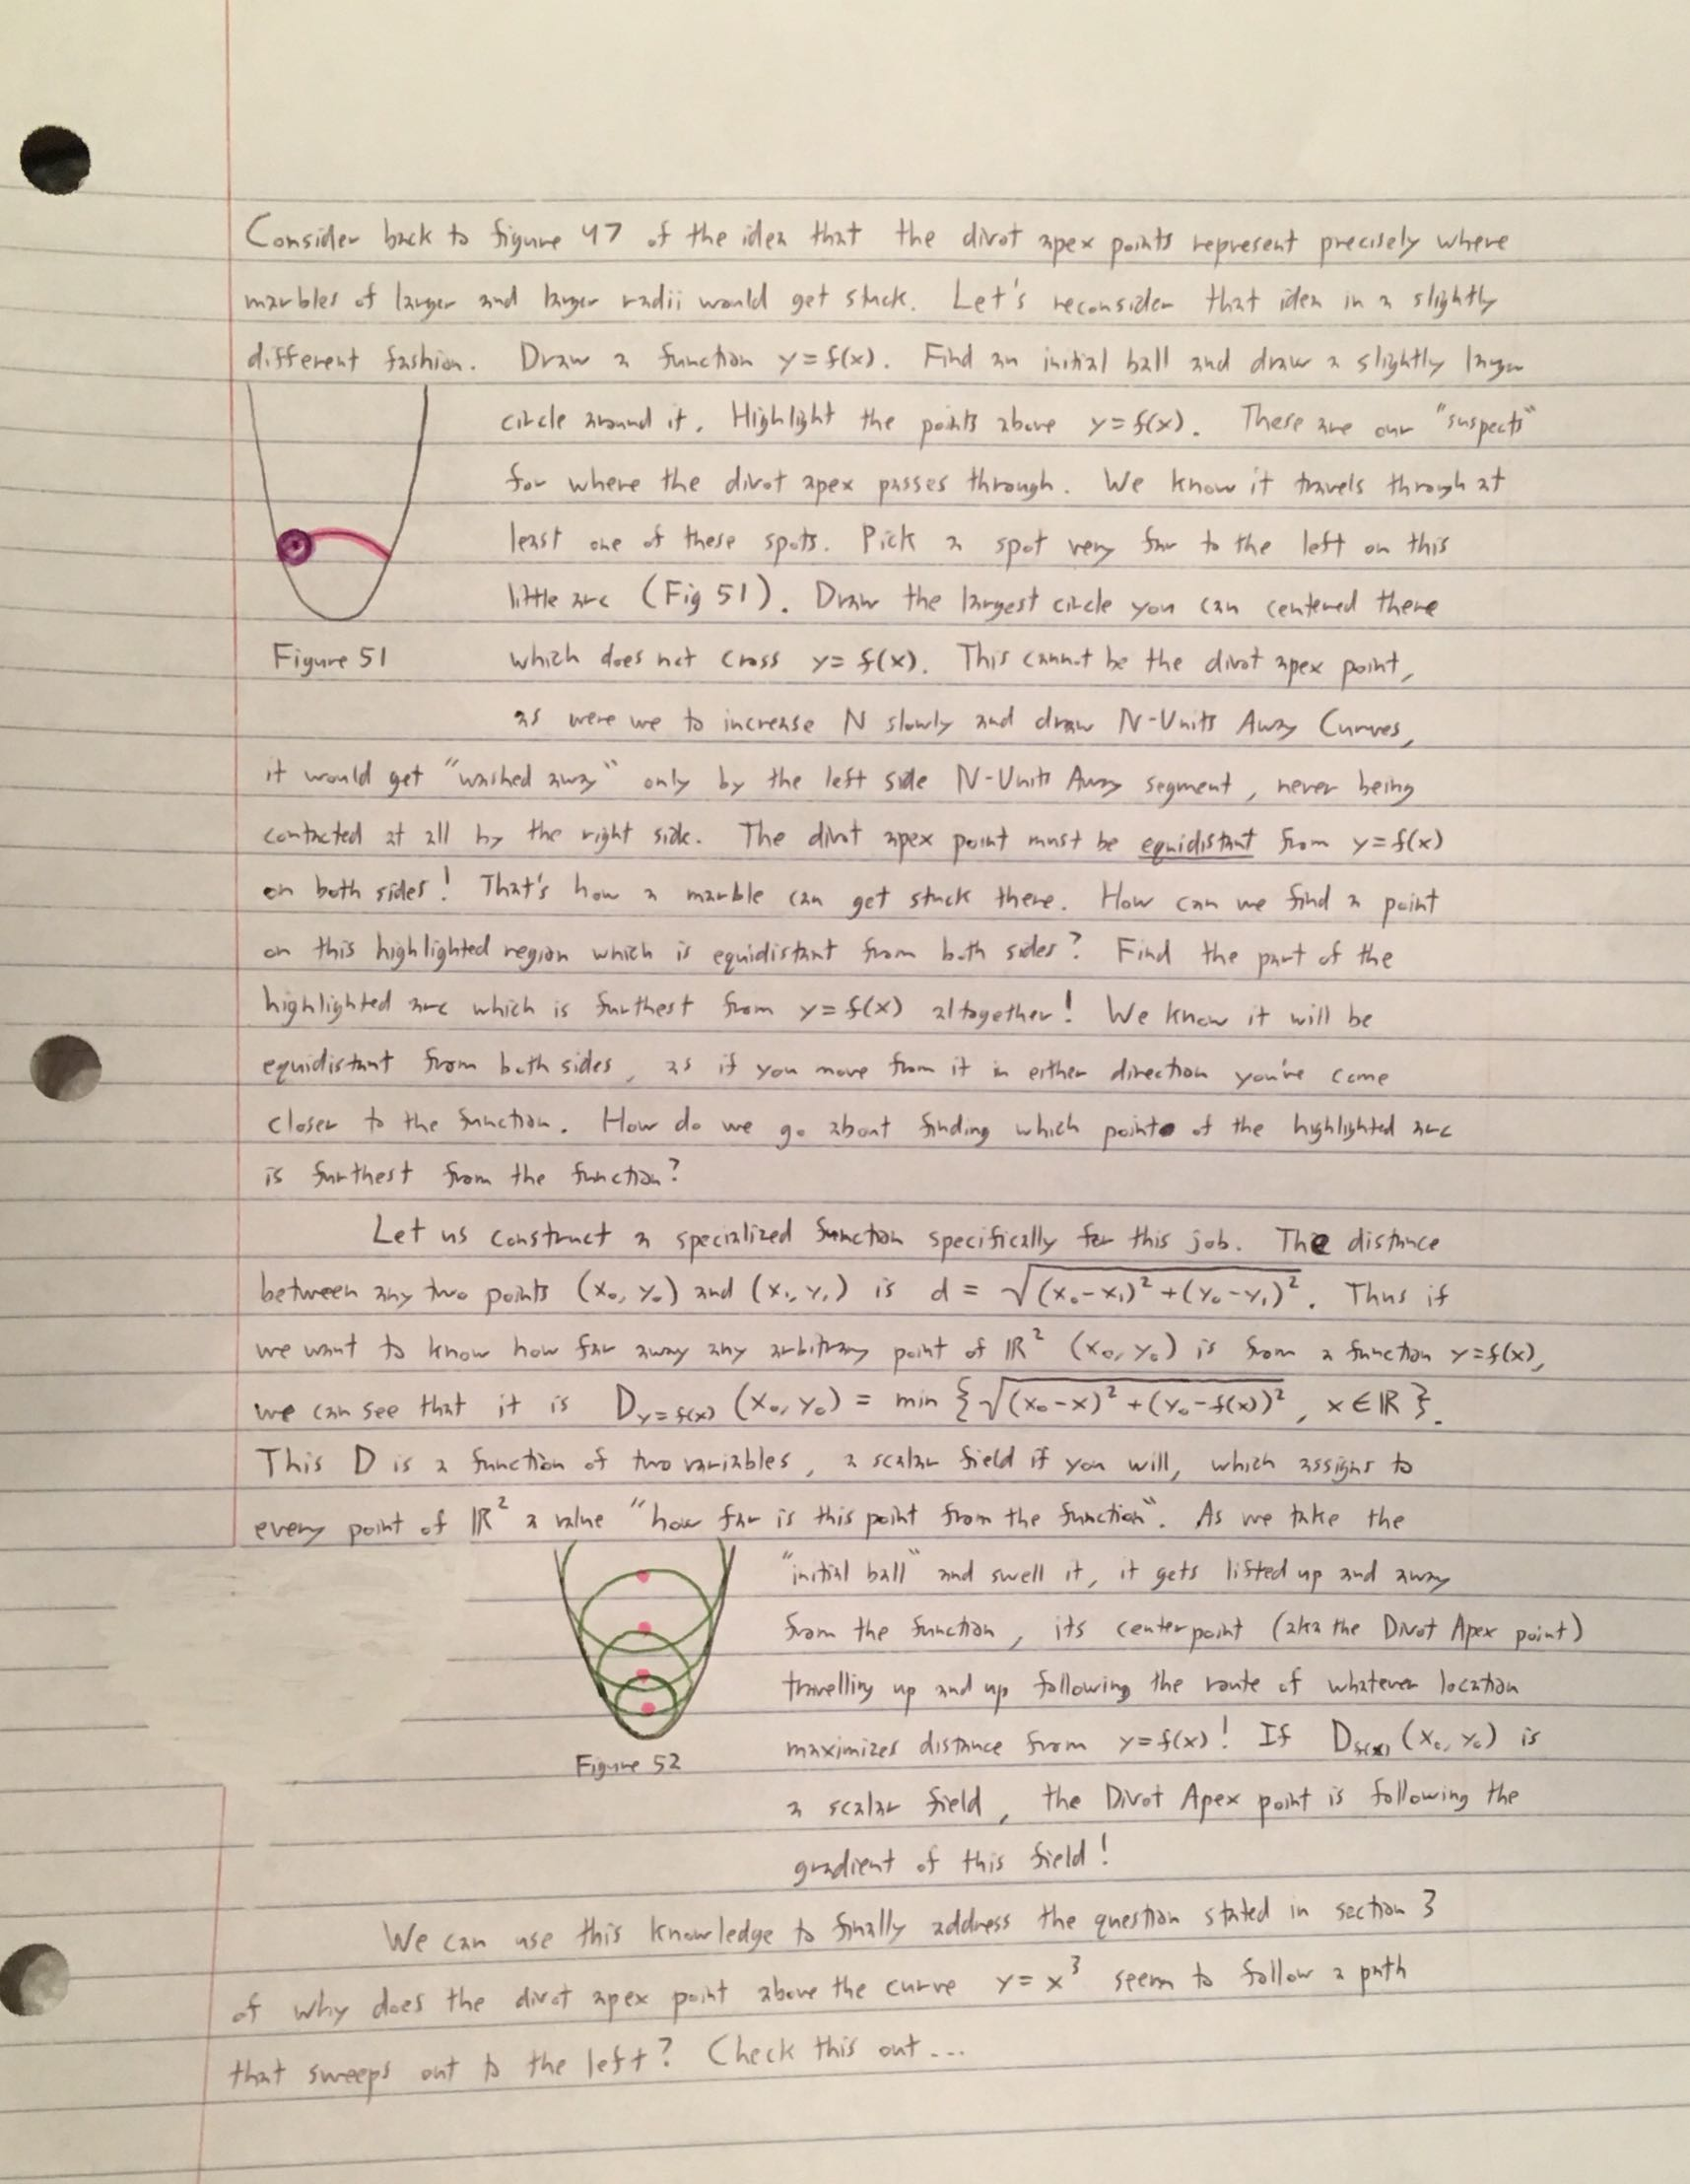
\includegraphics[width=.9\linewidth]{solving-divot-paths-img/Fig 12-51.png}
  \caption{Caption}
  \label{fig:fig12-51}
\end{wrapfigure}

Consider back to figure $\ref{fig:fig12-47}$ of the idea that the divot apex points represent precisely where marble of larger and larger radii would get stuck. Let's reconsider that idea in a slightly different fashion. Draw a function $y = f(x)$. Fins an initial ball and draw a slighlty larger circle arounf it. Highlight the points above $y = f(x)$. These are our ``suspects'' for where the divot apex passes through. We know it travels through at least one of these spots. Pick a spot very far to the left on this little arc (Fig $\ref{fig:fig12-51}$. Draw the largest circle you centered there which does not cross $y = f(x)$. This cannot be the divot apex point, as were we to increase $N$ slowly and draw $N$-Units Away segment, never being contacted at all by the right sick. The divot apex point must be \textit{equidistant} from $y = f(x)$ on both sides! That's how a marble can get stuck there. How can we find a point on this highlighted region which is equidistant from both sides? Find the part of the highlighted arc which is furthest from $y = f(x)$ altogether! We know it will be equidistant from both sides, as if you move from it in either direction you're come closer to the function. How do we go about finding which point of the highlighted arc is furthest from the function?

Let us construct a specialized function specifically for this job. The distance between any two points $(x_0, y_0)$ and $(x_1, y_1)$ is $d = \sqrt{(x_0 - x_1)^2 + (y_0 - y_1)^2}$, Thus if we want to know how far away any arbitrary points of $\mathbb{R}^2$ $(x_0, y_0)$ is from a function $y = f(x)$. we can see that it is $D_{y = f(x)}(x_0, y_0) = min \{ \sqrt{x_0 - x_1)^2 + (y_0 - y_1)^2} | x \in \mathbb{R} ^ 2$,

\begin{wrapfigure}{l}{0.25\textwidth}
  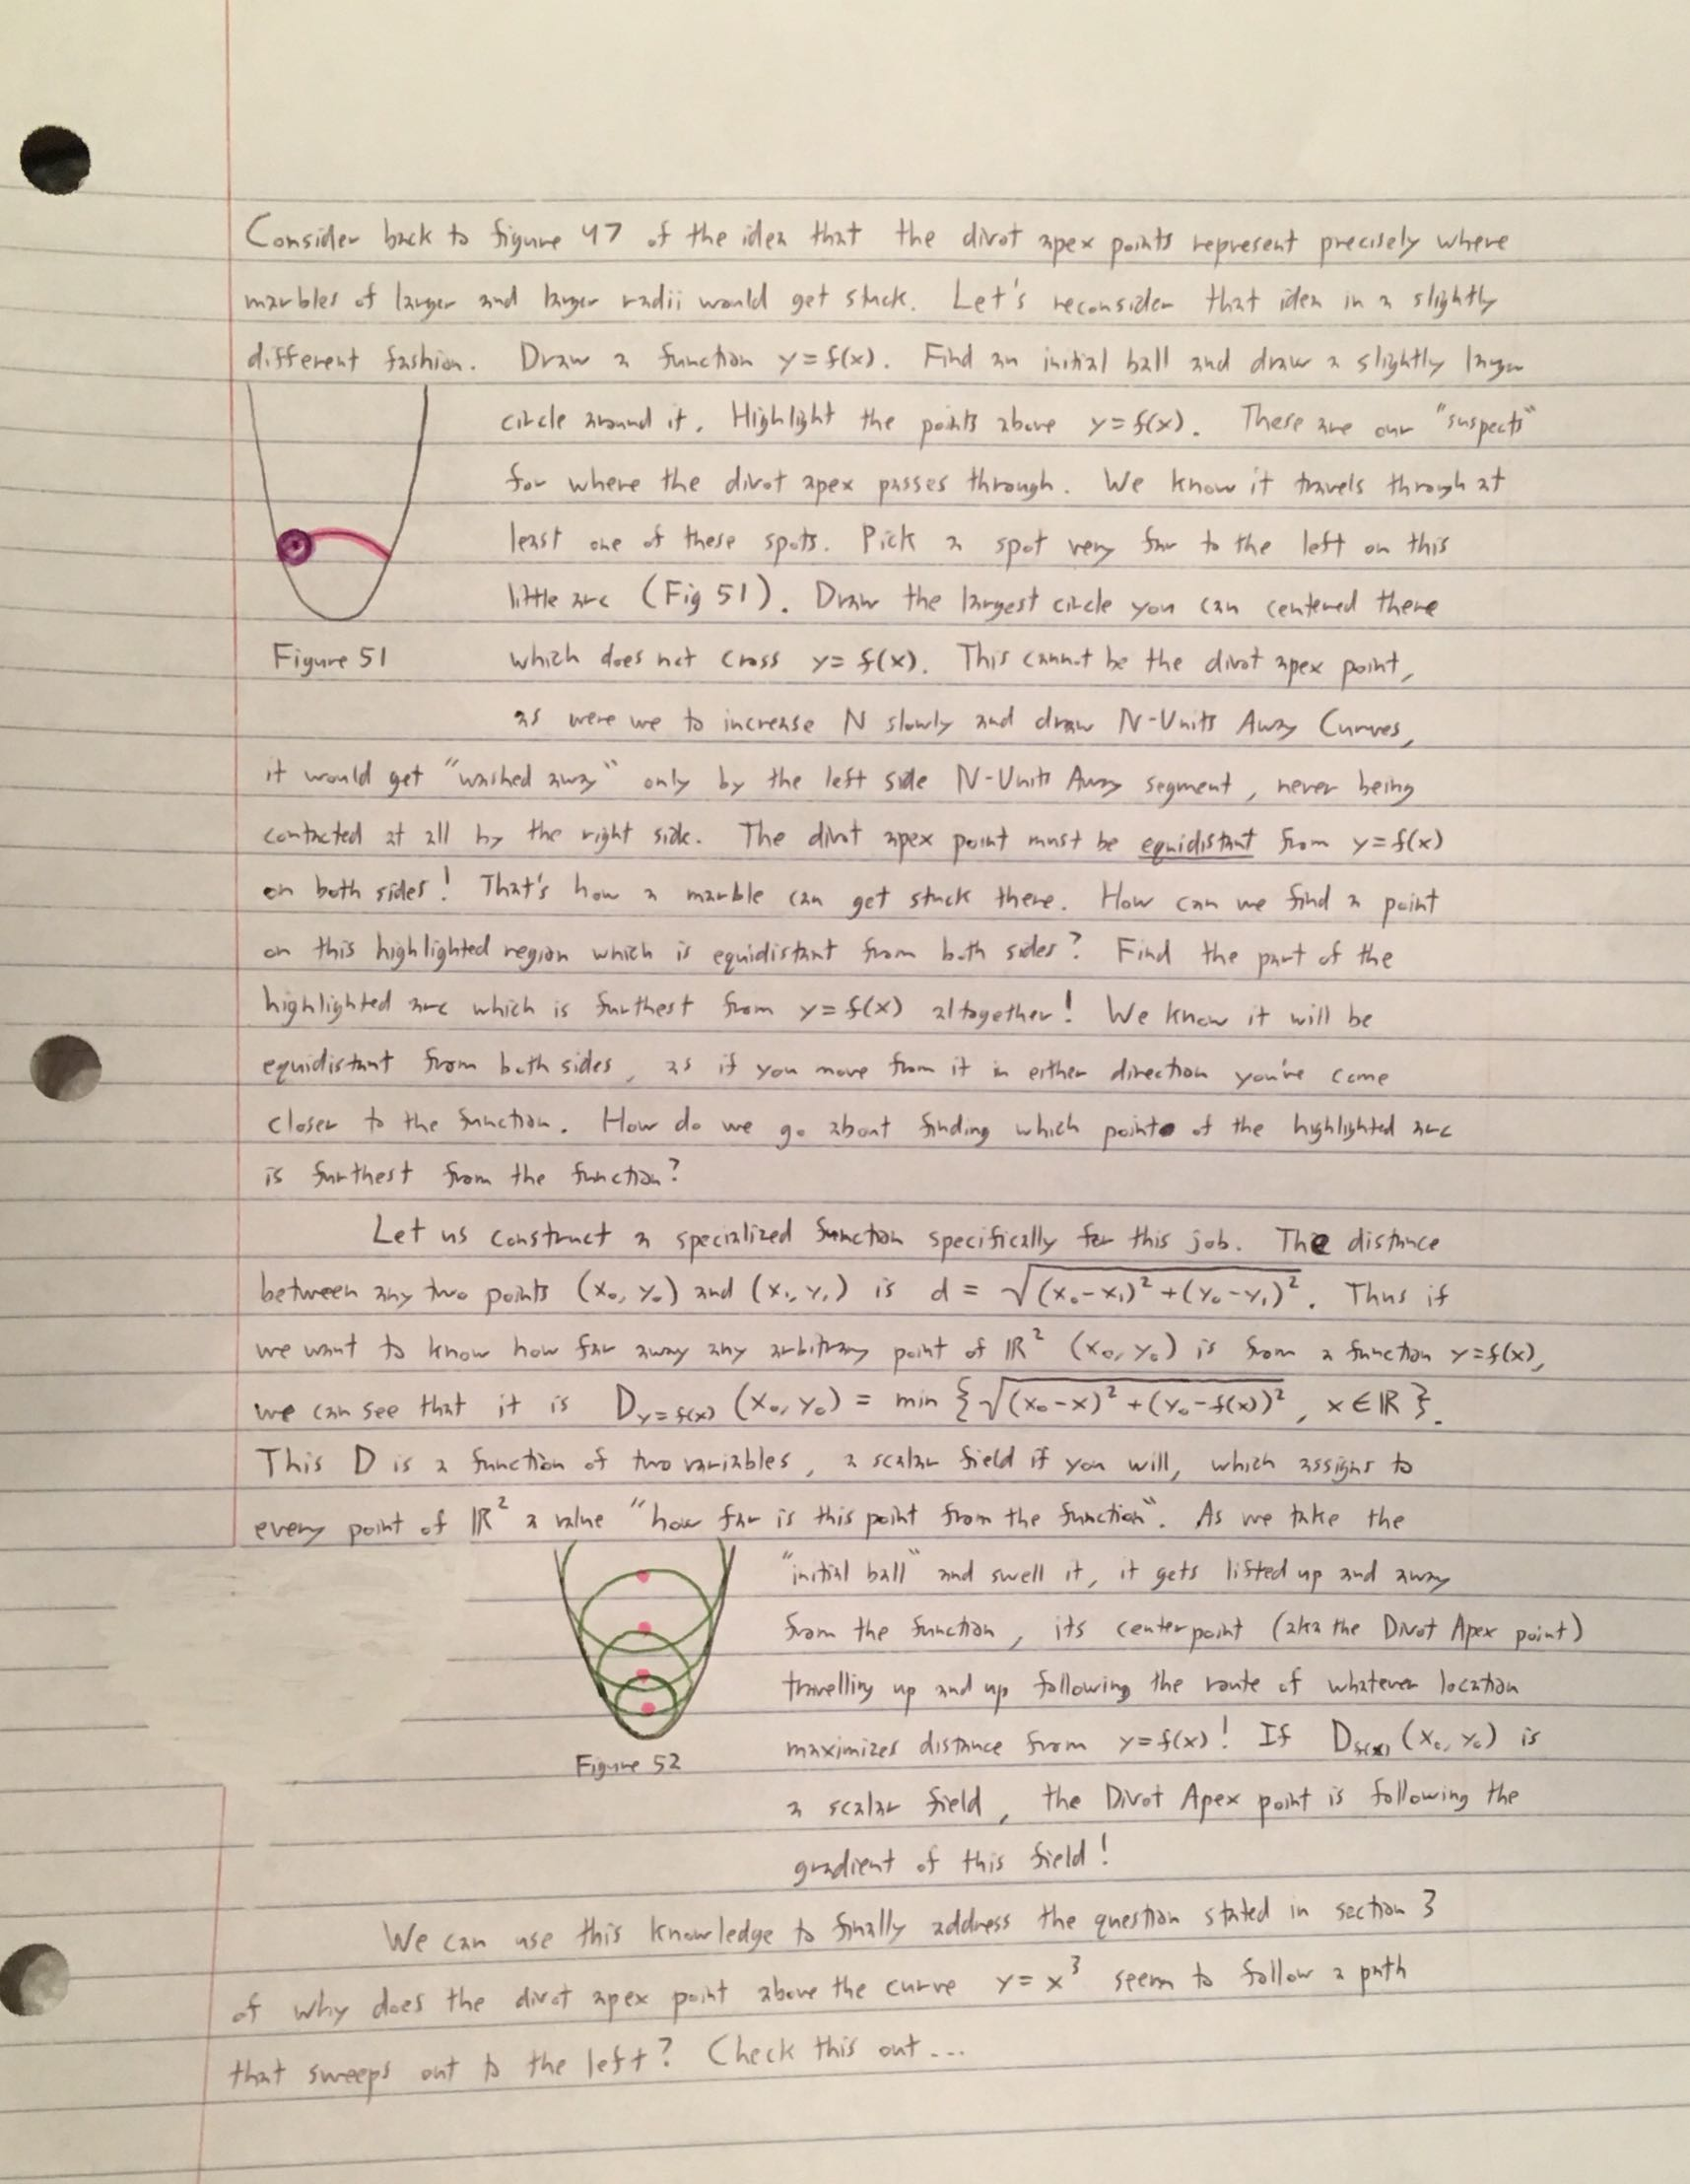
\includegraphics[width=.9\linewidth]{solving-divot-paths-img/Fig 12-52.png}
  \caption{Caption}
  \label{fig:fig12-52}
\end{wrapfigure}

This $D$ is a function of two variables, a scalar field if you will, which assigns to every point of $\mathbb{R} ^ 2$ a value ``how far is this point from the function''. As we take the ``initial ball'' and swell it, it gets lifted up and away from the function, its centerpoint (aka the Divot Apex point) travelling up and up following the route of whatever location maximizes distance from $y = f(x)$! If $F_{f(x)}(x_0, y_0)$ is a scalar field, the Divot Apex point is following the gradient of this field!

We can use this knowledge to finally address the question stated in section 3 of why does the divot apex point above the curve $y = x^3$ seem to follow a path that sweeps out to the left? Check this out...

\newlist{steps}{enumerate}{1}
\setlist[steps, 1]{label = Step \arabic*:}

\begin{wrapfigure}{l}{0.25\textwidth}
  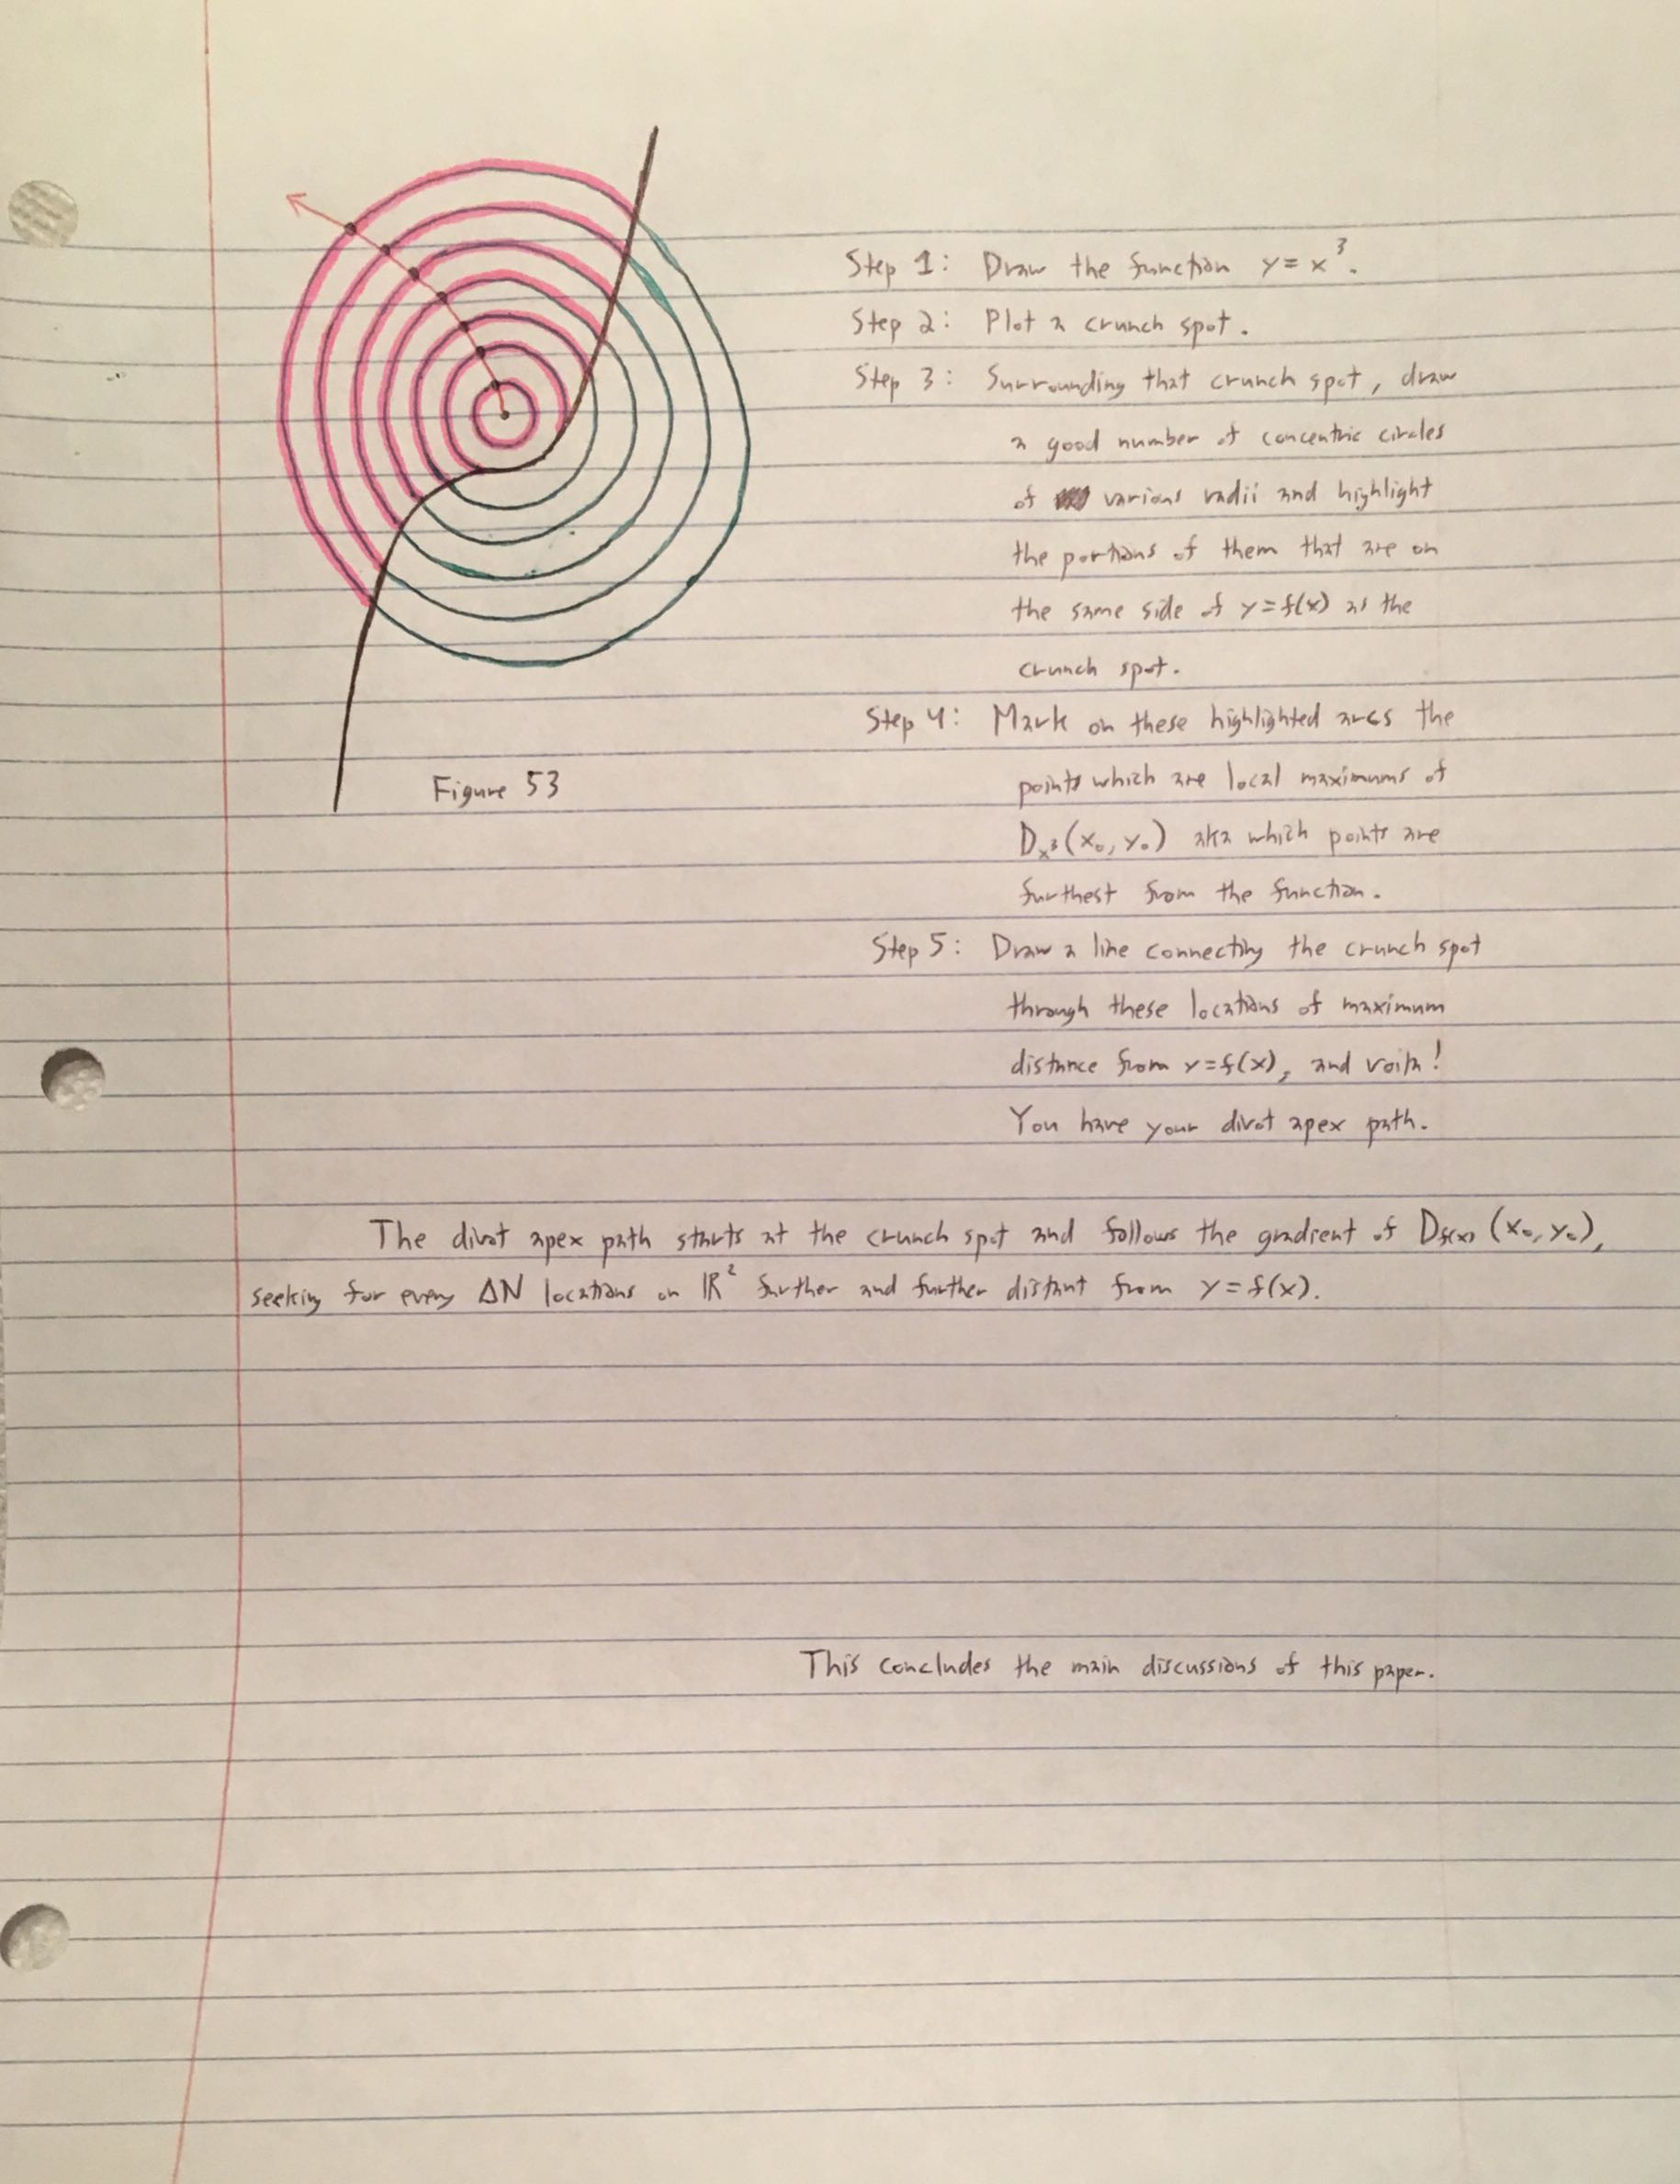
\includegraphics[width=.9\linewidth]{solving-divot-paths-img/Fig 12-53.png}
  \caption{Caption}
  \label{fig:fig12-53}
\end{wrapfigure}

\begin{steps}
  \item Draw the function $y = x ^ 3$
  \item Plot a crunch spot
  \item Surrounding that crunch spot, draw a good number of concentric circles of various radii and highlight the portions of them that are on the same side of $y = f(x)$ at the crunch spot.
  \item Mark on these highlighted arcs the points which are local maximums of $D_{x^3}(x_0, y_0)$ aka which points are furthest from the function.
  \item Draw a line connecting the crunch spot through these locations of maximum distance from $y = f(x)$, and voila! You have your divot apex path.
\end{steps}

The divot apex path starts at the crunch spot and follow the gradient of $D_{f(x)}(x_0, y_0)$, seeking for every $\Delta N$ location on $\mathbb{R} ^ 2$ further and further distant from $y = f(x)$.

This concludes the main discussions of this paper.